% !TeX program = pdflatex
\documentclass[preprint,12pt]{elsarticle}
\journal{Computer Networks}
\usepackage{amsmath,amssymb,amsthm,booktabs,graphicx,algorithm,algorithmic,multirow}
\usepackage{float}
\newtheorem{proposition}{Proposition}
\emergencystretch=1.5em
\usepackage{tikz}
\usetikzlibrary{arrows.meta,positioning,fit,calc}

\begin{document}
\begin{frontmatter}
\title{FedRAS: Deadline-Aware Rank Scheduling for Federated LoRA in Mobile Edge Networks}
\author[inst1,inst2,inst3]{Wenyu Ma}
\author[inst1,inst2,inst3]{Tao Hu\corref{cor1}}
\author[inst1,inst2,inst3]{Xinlei Liu}
\cortext[cor1]{Corresponding author}
\ead{hutaondsc@163.com}
\address[inst1]{Information Engineering University, Zhengzhou 450001, China}
\address[inst2]{Key Laboratory of Cyberspace Endogenous Safety and Security of Henan Province, Zhengzhou 450001, China}
\address[inst3]{Key Laboratory of Cyberspace Security, Ministry of Education of China, Zhengzhou 450001, China}

\begin{abstract}
Federated LoRA sharply reduces model update size, yet deploying it over mobile edge networks exposes a mismatch. The adaptation rank is a fixed hyperparameter while link capacity varies within every round, so high-rank updates may miss the deadline, whereas low-rank updates underuse stable links. We recast Federated LoRA scheduling as a joint client--rank assignment problem treating the rank as a network-visible resource determining update size, transmission time, and timely delivery, and we call the resulting mechanism FedRAS. Each round, FedRAS estimates a timely-delivery probability and a capacity gain per candidate rank, then selects clients and ranks to maximize expected useful updates under a budget and a participation cap. The resulting assignment is solved exactly by a pseudo-polynomial dynamic program, and heterogeneous ranks are aggregated by rank-masked averaging over frozen factors.

Trace-driven experiments couple a real federated LoRA trainer on non-IID CIFAR-10, CIFAR-100, and MNIST with a 500-client scheduling simulator, external baselines, ablations, and sensitivity analyses. Under nominal deadlines every rank preserves backbone accuracy while full-parameter updates spend $2.2\times$ the bytes for no gain. Under deadline stress FedRAS downshifts to delivered rank 13.5, matches fixed rank 16, and saves 14\% of bytes, confirmed over ten seeds at $p{=}0.002$, while 96\% of full-parameter updates miss the deadline and simulations show 73\% fewer timely updates than rank-16 LoRA. The dynamic program attains the per-round optimum, beating greedy scheduling by up to 10\% in binding regimes at 33--836\,ms solver cost. No universal accuracy dominance is claimed; the results delineate when rank adaptation pays for itself in timeliness and bytes.
\end{abstract}

\begin{keyword}
Federated LoRA \sep Mobile edge computing \sep Adaptive rank \sep Deadline scheduling \sep Wireless federated learning
\end{keyword}
\end{frontmatter}

\section{Introduction}
\label{sec:intro}

Mobile edge networks increasingly host federated learning (FL) workloads in which heterogeneous clients such as smartphones, vehicles, UAV terminals, and satellite-connected devices collaborate on a shared model without exposing raw data \cite{mcmahan2017fedavg,kairouz2021advances,liu2018sagin,mahboob2024ntn}. The dominant cost in such systems is the uplink. Full-parameter model updates saturate wireless capacity, drain client energy, and frequently miss round deadlines when links degrade during handover or outage, as reported for ground, aerial, and satellite segments \cite{razmi2022ground,tang2023flsagin,qin2024dfrl,ribero2023intermittent}. Low-rank adaptation (LoRA) has therefore become an attractive transmission format for FL, because only two small factor matrices per adapted layer are communicated instead of the full weight delta \cite{hu2022lora,babakniya2023slora,zhang2024fedit}.

Existing Federated LoRA systems, however, treat the rank $r$ as a fixed model hyperparameter, shared by all clients and all rounds. This convention ignores a scheduling dimension that is directly visible to the network. The rank determines the number of transmitted parameters and hence the transmission time. On a time-varying link, a larger rank raises the probability that the update misses the round deadline $\tau$, while a conservative small rank underuses a stable link and limits how much adaptation each round can carry. In other words, the LoRA rank is a network scheduling variable and not only a learning parameter. A scheduler that can choose the rank per client and per round, admitting a handover-prone client at $r{=}4$ while letting a broadband client transmit $r{=}16$, converts link heterogeneity from a source of deadline failures into a controllable trade-off between adaptation capacity and timely delivery.

Making this idea precise requires answering three questions that, to our knowledge, have not been addressed jointly. First, how should the timely-delivery probability of a rank-$r$ update be modeled from observable link state, given that the update size itself depends on $r$? Second, how should the per-round joint client--rank assignment be solved under a communication budget and a participation cap, and what does exactness cost? Third, does rank adaptation actually pay off end to end in delivered bytes, timeliness, and accuracy when evaluated with a real federated LoRA trainer rather than only an abstract utility model?

\subsection{Contributions}
This paper answers these questions with a complete scheduling stack, comprising a delivery model, an exact solver, a deployable rank-adaptation rule, and a two-tier experimental evaluation. We call the resulting mechanism FedRAS. We make four contributions.

\begin{itemize}
\item \textbf{Deadline-aware client--rank model.} We formulate per-round Federated LoRA scheduling as a joint assignment problem in which each admitted client also selects a rank. The model links the rank to update bytes, processing and transmission time, a mobility- and deadline-conditioned timely-delivery probability $P_{\mathrm{on}}(r)$, and a saturating adaptation-capacity gain $G(r)$, so that expected useful updates can be optimized rather than accuracy or reliability alone. Sections~\ref{sec:model} and \ref{sec:problem} develop this model.
\item \textbf{Exact dynamic-programming scheduler.} We show that the estimated per-round problem is a multiple-choice knapsack with an admission cap, derive an exact pseudo-polynomial dynamic program of complexity $O(|\mathcal D| K B_{\max}|\mathcal R|)$, and prove its conditional per-round optimality. Sections~\ref{sec:solver} and \ref{sec:dp_study} also quantify the optimality gaps of greedy heuristics, up to 10\% in binding regimes, and the solver runtime of 33 to 836\,ms at 500 clients.
\item \textbf{Heterogeneous-rank aggregation.} We aggregate simultaneously arriving updates of different ranks by rank-masked averaging over frozen random factors. Freezing the $A$ factor at a shared initialization \cite{sun2024ffalora} makes factor averaging exact on the induced updates at every rank slice and stabilizes training. The rank mask prevents low-rank updates from diluting high-rank coordinates in the shared $r_{\max}$ coordinate system \cite{wang2024flora,babakniya2023slora}. Proposition~\ref{prop:agg} in Section~\ref{sec:aggregation} states the exactness properties and their limits.
\item \textbf{Two-tier evaluation with a real trainer.} The first tier is a real federated LoRA trainer on non-IID CIFAR-10, CIFAR-100, and MNIST, with adapters on all convolutional and head layers, five seeds, and 40 rounds. The second tier is a 500-client, 150-round scheduling simulator over nine deadline, budget, mobility, and scale regimes. Under a 0.25\,s deadline, FedRAS downshifts to a delivered mean rank of 13.5, matches fixed rank 16, and saves 14\% of bytes, while full-parameter updates aggregate only 0.4 of 10 updates per round. In the 500-client simulation, full-parameter updates deliver 73\% fewer timely updates than rank-16 LoRA at $2.2\times$ the bytes, with no accuracy gain anywhere. The evaluation further covers external baselines, component ablations, sensitivity studies, and a direct trainer comparison of full scheduling and fair cohort in Section~\ref{sec:eval}.
\end{itemize}

A preliminary poster version of this work studied joint client--protection scheduling for federated learning in space--air--ground mobile networks \cite{ma2026mswim}. The present article substantially reformulates that line of work around a different schedulable resource. It replaces compression-and-protection policies with the LoRA rank as the per-client decision variable. It introduces the MB-to-Mbit delivery hazard and the saturating capacity model of Section~\ref{sec:model}, replaces the heuristic admission-and-repair procedure with an exact client--rank dynamic program, and adds frozen-factor rank-masked aggregation for heterogeneous ranks. It also reports a new two-tier evaluation comprising a real federated LoRA trainer, a 500-client scheduling simulator, and a solver exactness study. Accordingly, all numerical results in this article come from the revised formulation and implementation and are not comparable with the preliminary version.

We deliberately report accuracy, timely ratio, and transmitted bytes separately, and we claim no universal accuracy dominance. With a frozen pretrained backbone, rank choice should preserve accuracy, and its value must be demonstrated on the network side. This framing keeps every claim testable.

The remainder of this paper is organized as follows. Section~\ref{sec:related} reviews related work. Section~\ref{sec:model} introduces the system model. Section~\ref{sec:problem} formulates the scheduling problem and Section~\ref{sec:solver} presents the solver and the aggregation scheme. Section~\ref{sec:eval} reports the evaluation, Section~\ref{sec:discussion} discusses limitations, and Section~\ref{sec:conclusion} concludes.

\section{Related work}
\label{sec:related}

\subsection{Parameter-efficient and federated LoRA}
LoRA freezes a pretrained backbone and learns low-rank weight increments $\Delta W = BA$ \cite{hu2022lora}; because $B$ is initialized at zero, the adapted model starts exactly at the backbone. Federated LoRA trains such adapters across clients: SLoRA \cite{babakniya2023slora} demonstrated sparsity-aware averaging of sparse LoRA updates, FedIT \cite{zhang2024fedit} federated instruction tuning with low-rank local updates, and heterogeneous-rank aggregation was studied by stacking aligned factors \cite{wang2024flora} and by model-heterogeneous personalization \cite{yi2024fedlora}.

FFA-LoRA \cite{sun2024ffalora} froze one factor at its random initialization and showed that this improves stability in privacy-preserving federated fine-tuning. We adopt the same frozen-factor property for a stronger reason. When the frozen factor is identical across clients, averaging the trainable factor is exactly averaging the update at every rank slice, as Proposition~\ref{prop:agg} shows. It thereby removes the factor-rotation inconsistency that we show empirically to destabilize joint A/B training. Section~\ref{sec:aggregation} develops this aggregation.

Closest to our setting, SA-FedLoRA schedules the rank over rounds with a simulated-annealing schedule that is oblivious to network state \cite{yang2024safedlora}, and FedSA-LoRA aggregates only the A factor while keeping B client-local, its asymmetry analysis identifying joint-factor averaging as the error-prone alternative \cite{guo2025fedsalora}. These works optimize learning-side objectives; none makes the rank a per-round network decision conditioned on link state and deadline. Section~\ref{sec:eval} compares against a faithful adaptation of the annealing schedule and against joint-factor averaging, the aggregation strategy that both FFA-LoRA and FedSA-LoRA argue against.

\subsection{Communication-efficient federated learning}
A broad literature reduces FL communication through sparsification, quantization, compressed sensing, and over-the-air aggregation \cite{oh2023fedqcs,oh2024fedvqcs,liu2023adaptivequant,kim2023beamforming,reisizadeh2020fedpaq,lin2018deep}. These mechanisms compress a given update. The scheduler we study instead chooses the structure of the update, that is, its rank, before compression, which couples the decision directly to transmission time and deadline feasibility. The capacity-gain and delivery models are therefore complementary to codec-level compression and can be combined with it at any selected rank.

\subsection{Client selection and deadline-aware scheduling}
Client selection improves FL efficiency by admitting useful clients under data, latency, and energy heterogeneity \cite{oort2021oort,chen2024clientselection,dong2024aoi,luo2021costeffective}. Deadline- and reliability-aware participation has been studied for mobile and non-terrestrial networks, where visibility windows, handover, and outage dominate participation \cite{razmi2022ground,tang2023flsagin,qin2024dfrl,ribero2023intermittent,han2024orchestrating}. These schedulers select which clients participate, and the update each client sends is assumed exogenous. Our evaluation includes an Oort-style utility selector \cite{oort2021oort} as a selection-level baseline, with the update-size decision kept fixed to isolate the effect of network-aware ranking. In our formulation the participation decision and the update-size decision are the same decision variable pair $(i, r)$, which is what makes the joint problem a multiple-choice knapsack rather than a top-$K$ selection.

\subsection{Positioning}
We do not claim any individual ingredient as new. To the best of our knowledge, the following combination has not previously appeared as a whole. It comprises the LoRA rank treated as a deadline-constrained network resource with an explicit MB-to-Mbit delivery hazard, an exact per-round client--rank assignment with quantified greedy gaps and solver cost, and validation of the resulting trade-offs with a real federated trainer in which adapters are placed on every block of the backbone, rather than only with synthetic utility curves. The claim is conditional on the surveyed literature of Section~\ref{sec:related} and on the evaluated setting.

\section{System model}
\label{sec:model}

\begin{figure}[H]
\centering
\resizebox{\columnwidth}{!}{%
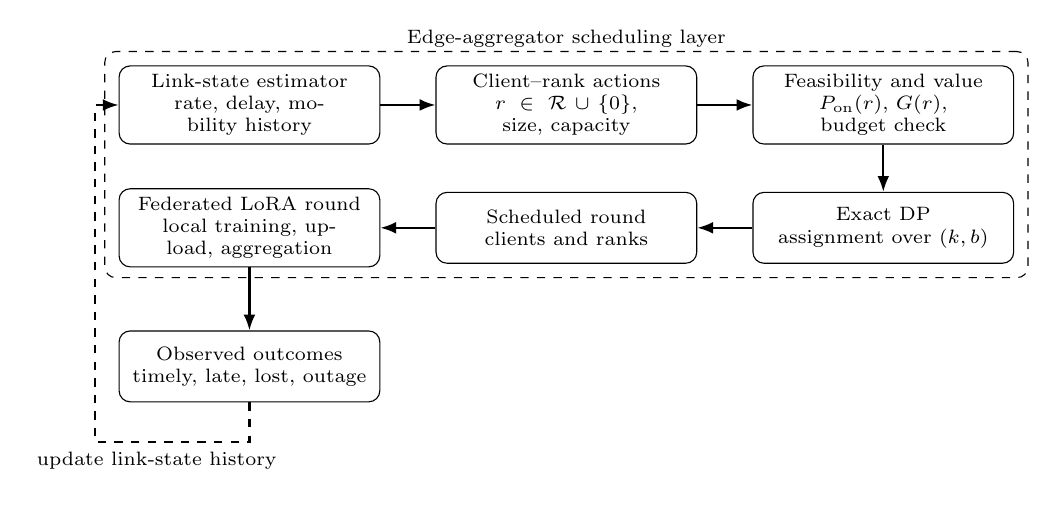
\begin{tikzpicture}[
  node distance=6mm and 7mm, >=Latex,
  box/.style={draw, rounded corners, align=center, minimum height=9mm, text width=31mm, font=\scriptsize, inner sep=3pt},
  flow/.style={-{Latex[length=2mm]}, thick},
  feedback/.style={-{Latex[length=2mm]}, dashed, thick}
]
\node[box] (estimate) {Link-state estimator\\rate, delay, mobility history};
\node[box, right=of estimate] (actions) {Client--rank actions\\$r\in\mathcal R\cup\{0\}$, size, capacity};
\node[box, right=of actions] (filter) {Feasibility and value\\$P_{\rm on}(r)$, $G(r)$, budget check};
\node[box, below=of filter] (dp) {Exact DP\\assignment over $(k,b)$};
\node[box, left=of dp] (assign) {Scheduled round\\clients and ranks};
\node[box, left=of assign] (fl) {Federated LoRA round\\local training, upload, aggregation};
\node[box, below=8mm of fl] (observe) {Observed outcomes\\timely, late, lost, outage};
\draw[flow] (estimate) -- (actions);
\draw[flow] (actions) -- (filter);
\draw[flow] (filter) -- (dp);
\draw[flow] (dp) -- (assign);
\draw[flow] (assign) -- (fl);
\draw[flow] (fl) -- (observe);
\coordinate (fb) at ($(fl.south)+(0,-4mm)$);
\draw[feedback] (observe.south) -- ++(0,-5mm) -| node[below, font=\scriptsize, pos=.3] {update link-state history} ($(estimate.west)+(-3mm,0)$) -- (estimate.west);
\node[draw, dashed, rounded corners, fit=(estimate)(actions)(filter)(dp)(assign), inner sep=5pt,
      label={[fill=white, inner sep=1pt, font=\scriptsize]above:Edge-aggregator scheduling layer}] {};
\end{tikzpicture}%
}
\caption{Round pipeline of FedRAS. The edge aggregator jointly selects clients and LoRA ranks with an exact dynamic program; only observed transmission outcomes update the link-state history.}
\label{fig:architecture}
\end{figure}

\subsection{Mobile edge FL architecture}
We consider a mobile edge network in which an edge aggregator serves a client set
$\mathcal{D}=\mathcal{D}_g\cup\mathcal{D}_a\cup\mathcal{D}_s$ of ground clients $\mathcal{D}_g$, aerial and UAV clients $\mathcal{D}_a$, and satellite-connected clients $\mathcal{D}_s$. Ground links are comparatively stable, aerial links face frequent handover, and satellite links suffer long propagation delay, intermittent visibility, and outages \cite{mahboob2024ntn,razmi2022ground}. The aggregator holds the global model, schedules every round, and aggregates the timely updates. Fig.~\ref{fig:architecture} shows the resulting round pipeline. In every round the aggregator estimates the link states, constructs and filters the client--rank actions, and solves the assignment with the dynamic program of Section~\ref{sec:solver}. It then executes the federated round and feeds the observed delivery outcomes back into the link-state history.

\subsection{Federated LoRA rounds}
Let $w^t$ denote the frozen backbone broadcast at round $t$. Client $i$ trains LoRA factors $A_{i,\ell}$ and $B_{i,\ell}$ for the adapted layers $\ell\in\mathcal L$ with layer dimensions $d_\ell\times k_\ell$. The effective weight change is $\Delta W_{i,\ell}=B_{i,\ell}A_{i,\ell}$, limited to the first $r$ factor columns when the client is scheduled at rank $r$. A round then proceeds as follows. The aggregator broadcasts the backbone and the current adapter state. It observes the client link states and solves the client--rank assignment under the deadline, budget, and participation constraints. The admitted clients train locally and upload their rank-$r$ adapters before the deadline $\tau$. The aggregator aggregates the timely updates with data-size weights and updates its link-state history from the observed outcomes. Late or lost updates are discarded, because stale updates harm convergence stability in deadline-critical federated learning.

\subsection{Link, mobility, and delivery model}
At decision time each client exposes an observable state $x_i^t$ with the estimated uplink rate $\bar R_i^t$ in Mbps, the propagation delay $d_i^t$, the loss probability $p_i^t$, and mobility features such as the serving node, the velocity, and the link trend. The realized rate $R_i^t$, the handover event $H_i^t\in\{0,1\}$, and the packet-loss indicator $J_i^t$ are random and unknown at decision time. For an update of $B$ megabytes, the delivery time is
\begin{equation}
T_i^t(r)=T_{\rm train,i}(r)+T_{\rm proc,i}(r)+\frac{8\,B_i^t(r)}{R_i^t}+d_i^t+H_i^t\Delta d_h,
\label{eq:delivery}
\end{equation}
where the factor 8 converts megabytes to Mbit against an Mbps rate and a deadline in seconds, and $\Delta d_h$ is the handover delay penalty. The training and processing times $T_{\rm train}$ and $T_{\rm proc}$ grow weakly with $r$. Timely delivery is the joint event
\begin{equation}
P_{\rm on,i}^t(r)=\Pr\!\left(T_i^t(r)\le\tau,\;J_i^t=0\mid x_i^t\right),
\label{eq:pon}
\end{equation}
estimated before the update exists, so the assignment leaks no future outcome into the decision.

Our implementation estimates \eqref{eq:pon} with the hazard-form surrogate
\begin{equation}
\hat P_{\rm on,i}^t(r)=\exp\!\big(-\mu_i^t\big)\exp\!\Big(-\frac{8\,B_i^t(r)}{\bar R_i^t\,\tau}\Big).
\label{eq:hazard}
\end{equation}
The first factor covers the non-transmission terms of \eqref{eq:delivery}. Its exponent $\mu_i^t\ge 0$ is the round-integrated mobility intensity of the client, a dimensionless quantity that absorbs handover, outage, packet loss, and training or processing overruns, so $e^{-\mu_i^t}$ is the probability of surviving the round without such a failure. The second factor is a transmission-time surrogate. With $m=8B/\bar R$ the mean transmission time at the estimated rate, the factor $\exp(-m/\tau)$ matches the exponential-service success probability $1-e^{-\tau/m}$ to first order in the regime $m\ll\tau$ that matters for scheduling. It never overestimates that probability anywhere, since $e^{-x}+e^{-1/x}\le 1$ for all $x=m/\tau>0$.

In the experiments, $\mu_i^t$ follows the mobility model of Section~\ref{sec:eval} and is treated as observable link state at decision time, which makes the predictor idealized. The scheduler accepts any plug-in predictor in place of \eqref{eq:hazard}. Section~\ref{sec:eval} measures the reliability curve of \eqref{eq:hazard}, its expected calibration error, and the scheduling cost of mis-calibration. Section~\ref{sec:discussion} outlines per-client calibration from observed delivery outcomes for deployment.

\subsection{Rank-dependent update size and capacity}
With $b$ bits per parameter, the payload of a rank-$r$ LoRA update is
\begin{equation}
B_i^t(r)=\frac{b}{8}\;r\!\!\sum_{\ell\in\mathcal L}\big(d_\ell+k_\ell\big)+B_{\rm meta},
\label{eq:size}
\end{equation}
in MB, where $B_{\rm meta}$ covers headers and metadata. Rank is therefore a network-visible resource. It scales both the adaptation capacity and the transmission time. We model the useful contribution of a delivered rank-$r$ update with the saturating capacity gain
\begin{equation}
G_i^t(r)=\pi_i^t\,\sqrt{\min(r,r_{\max})/r_{\max}},
\label{eq:cap}
\end{equation}
where $\pi_i^t$ is a per-client contribution prior in the spirit of Oort-style utility \cite{oort2021oort}, built from the data size and a recency-weighted update norm. The width $r_{\max}$ is the factor width provisioned at all clients. The square root encodes diminishing returns of rank. The saturation at $r_{\max}$ reflects that wider factors add payload but no expressible capacity once the provisioned width is reached. The full-parameter FedAvg updates of our experiments operate exactly in this regime.

\section{Deadline-aware client--rank scheduling}
\label{sec:problem}

Each round, the aggregator decides $a_i^t\in\{0\}\cup\mathcal R$, where $a_i^t=0$ means client $i$ does not participate and $a_i^t=r$ schedules it at rank $r$. The per-round problem is
\begin{equation}
\max_{\{a_i^t\}}\;\sum_{i\in\mathcal D}\mathbf 1\{a_i^t>0\}\,G_i^t(a_i^t)\,P_{\rm on,i}^t(a_i^t)
\label{eq:objective}
\end{equation}
\begin{equation}
\text{s.t.}\quad \sum_i B_i^t(a_i^t)\le B_{\max},\qquad \sum_i\mathbf 1\{a_i^t>0\}\le K .
\label{eq:constraints}
\end{equation}
The objective counts the expected useful delivered updates rather than raw accuracy or link reliability, under the communication budget $B_{\max}$ and the participation cap $K$. Choosing the largest feasible rank everywhere is not optimal. Increasing $r$ raises $G$ sublinearly but increases $B$ linearly and lowers $P_{\rm on}$, so interior ranks dominate on slow links and under tight deadlines. The evaluation reports accuracy, timely ratio, and bytes separately, which keeps every claim falsifiable.

Two deployment variants are evaluated. In the full-scheduling variant, the aggregator solves \eqref{eq:objective} and \eqref{eq:constraints} over all clients, and Section~\ref{sec:dp_study} studies it at 500-client scale. The fair-cohort variant is the one used in the trainer. It samples the cohort uniformly at random, as standard cross-device FL does for fairness, and then applies, under the budget, the FedRAS rank rule $r_i^\star=\arg\max_r\, G_i^t(r)P_{\rm on,i}^t(r)$ to every admitted client. Section~\ref{sec:dpvfair} compares the two variants end to end in the trainer, and the solver study quantifies their objective gap at scale.

\section{Exact solver and heterogeneous-rank aggregation}
\label{sec:solver}

\subsection{Dynamic program}
Problem \eqref{eq:objective}--\eqref{eq:constraints} is a multiple-choice knapsack with an additional cardinality constraint. For a budget discretized into unit steps, let $V_i(k,b)$ be the maximum expected useful-update value achievable from the first $i$ clients with $k$ admissions and $b$ budget units used. Initialize $V_0(0,0)=0$ and all other states to $-\infty$. The recurrence is
\begin{equation}
V_i(k,b)=\max\Big\{V_{i-1}(k,b),\;\max_{r\in\mathcal R}\big[V_{i-1}(k-1,b-B(r))+u_i(r)\big]\Big\},
\label{eq:dp}
\end{equation}
where $u_i(r)=G_i^t(r)P_{\rm on,i}^t(r)$. Backpointers recover the assignment.

\begin{proposition}[Per-round optimality]
For every reachable state $(k,b)$, recurrence \eqref{eq:dp} considers all mutually exclusive actions of client $i$, the skip action and admission at any feasible rank, and retains the best value. By induction on $i$, $V_i(k,b)$ is the exact optimum over the first $i$ clients. Hence $\max_{k\le K,b\le B_{\max}}V_{|\mathcal D|}(k,b)$, with backpointers, is a globally optimal solution of the estimated per-round problem \eqref{eq:objective}--\eqref{eq:constraints} on the discretized budget grid.
\end{proposition}
\begin{proof}
The admission indicator and the rank of each client are exclusive actions that affect the two resources additively. Admitting client $i$ at rank $r$ consumes one admission slot and $B(r)$ budget units and adds $u_i(r)$ value, independent of the other clients. The state $(k,b)$ therefore summarizes all interaction, and the standard interchange argument for the multiple-choice knapsack applies. Any optimal solution restricted to the first $i-1$ clients must itself be optimal for its state, which the recurrence maximizes.
\end{proof}

The complexity is $O(|\mathcal D|\,K\,B_{\max}|\mathcal R|)$ time on a grid of $B_{\max}$ unit steps and $O(KB_{\max})$ memory with rolling arrays. In our implementation the budget step is 0.05\,MB. Section~\ref{sec:dp_study} reports runtimes of 33--836\,ms for 500 clients, linear in the population up to 1000 clients. The complete per-round procedure appears in Algorithm~\ref{alg:scheduler}.

\begin{algorithm}[t]
\caption{FedRAS scheduling round}
\label{alg:scheduler}
\begin{algorithmic}[1]
\REQUIRE clients $\mathcal D$, ranks $\mathcal R$, cap $K$, budget $B_{\max}$, deadline $\tau$, states $\{x_i^t\}$
\ENSURE admitted set and assigned ranks
\STATE Estimate $\hat P_{\rm on,i}^t(r)$ by \eqref{eq:hazard} and $G_i^t(r)$ by \eqref{eq:cap} for all $i,r$
\STATE Initialize $V_0(0,0)=0$; other DP states to $-\infty$
\FOR{each client $i\in\mathcal D$}
  \FOR{$k=0,\dots,K$ and each budget state $b$}
    \STATE Apply skip and every feasible rank transition of \eqref{eq:dp}
    \STATE Store the maximizing action as a backpointer
  \ENDFOR
\ENDFOR
\STATE Backtrack from $\max_{k,b} V_{|\mathcal D|}(k,b)$; return the client--rank assignment
\STATE Execute the round; aggregate timely rank-masked updates (Section~\ref{sec:aggregation}); update link-state history
\end{algorithmic}
\end{algorithm}

\subsection{Rank-masked aggregation with frozen factors}
\label{sec:aggregation}
Clients scheduled at different ranks deliver factors of different active widths in a shared $r_{\max}$ coordinate system. We state the aggregation for one adapted layer, and the construction repeats per layer. Client $i$ delivers its update with data weight $n_i$, the number of its local samples, and delivered rank $r_i$. The factor $A$ is frozen at the shared server-side initialization and is identical at every client \cite{sun2024ffalora}. The induced update is therefore $\Delta W_i=B_iA$ with $B_i\in\mathbb R^{d\times r_{\max}}$ and $A\in\mathbb R^{r_{\max}\times k}$, and a rank-$r_i$ update activates only the first $r_i$ factor columns, $\Delta W_i=\sum_{j\le r_i}\big[B_i\big]_{:,j}\big[A\big]_{j,:}$.

Jointly trained factor pairs $(A_i,B_i)$ are identifiable only up to invertible transforms, so separately averaged factors need not average the updates at all. Section~\ref{sec:eval} quantifies this failure mode in an ablation.

\textbf{Rank-masked averaging.} The server zero-pads every delivered $B_i$ outside its active coordinates and averages each coordinate over the clients that activate it,
\begin{equation}
\bar B_{:,j}=\frac{1}{W_j}\sum_{i:\,r_i\ge j} n_i\,\big[B_i\big]_{:,j},
\qquad
W_j=\sum_{i:\,r_i\ge j} n_i ,
\label{eq:maskavg}
\end{equation}
while the frozen factor aggregates to itself, $\bar A=A$. The server then applies momentum per factor tensor. With $\Delta^t=\bar B-S^{t-1}$, the velocity and state update as $v^t=\beta\,v^{t-1}+(1-\beta)\,\Delta^t$ and $S^t=S^{t-1}+v^t$, with $\beta=0.3$ damping client-sampling and link noise.

\begin{proposition}[Exactness of frozen-factor aggregation]
\label{prop:agg}
Under \eqref{eq:maskavg} with shared frozen $A$, first, for every coordinate $j$, the $j$-th rank slice of the aggregated update, $\bar B_{:,j}\big[A\big]_{j,:}$, equals the data-weighted average $\frac{1}{W_j}\sum_{i:\,r_i\ge j} n_i\,\big[B_i\big]_{:,j}\big[A\big]_{j,:}$ of the $j$-th rank slices of the induced updates of the clients active at level $j$.
Second, if a single global normalizer $W=\sum_i n_i$ is used at every coordinate instead, the aggregate is exactly the unified data-weighted average of the induced updates, $\bar BA=\frac{1}{W}\sum_i n_i B_iA$, but every slice above the smallest delivered rank shrinks by the factor $W_j/W\le 1$, a dilution of the high-rank coordinates. Third, the two aggregators coincide if and only if all delivered ranks are equal.
\end{proposition}
\begin{proof}
The first two parts follow from linearity. For frozen shared $A$, multiplying a weighted sum of $B$-coordinates by $\big[A\big]_{j,:}$ converts it into the same weighted sum of the matching update slices, and the two normalizers differ only in $W_j$ versus $W$. The product $\bar BA=\sum_j\bar B_{:,j}\big[A\big]_{j,:}$ collects the slices. The third part holds because $W_j=W$ for every active $j$ if and only if $r_i=\max_k r_k$ for all admitted $i$ with $n_i>0$.
\end{proof}

Proposition~\ref{prop:agg} delimits what masked averaging is. It averages the induced updates exactly per rank slice, with coordinate-dependent weights $n_i/W_j$, and it is not a unified weighted average of whole updates once ranks mix. We adopt it because the unified alternative shrinks precisely the high-rank coordinates that carry the extra capacity of high-rank clients \cite{wang2024flora,babakniya2023slora}. At the adopted operating point the admitted clients often share one rank, and the two aggregators coincide by the third part. Freezing $A$ is what makes these statements possible, and it also stabilizes training. An elevated-learning-rate ablation in Section~\ref{sec:eval} shows a markedly deeper transient accuracy dip under joint A/B updates, while frozen-$A$ training holds a tighter accuracy envelope across all 40 rounds.

\section{Performance evaluation}
\label{sec:eval}

The evaluation answers four questions. First, does rank adaptation preserve accuracy in a real federated LoRA trainer? Second, what do adaptive ranks buy in bytes and timeliness under deadline stress? Third, does the capacity-aware scheduler improve delivered useful updates at 500-client scale? Fourth, what is the price of exactness for the solver? A final group of studies probes the model assumptions themselves. The payload audit checks the byte accounting behind Section~\ref{sec:model}. The robustness and calibration studies perturb the delivery predictor and the capacity form of \eqref{eq:cap}. The grid sweep quantifies the budget discretization behind the solver.

\subsection{Experimental setup}
\textbf{Real trainer.} The trainer is implemented in PyTorch and runs on one A800 GPU. The backbone is a six-convolution BatchNorm CNN with channel progression 64/128/256, followed by two 256-wide linear layers. It is centrally pretrained with crop, flip, and erase augmentation, Nesterov momentum, weight decay, and cosine learning-rate decay, for 30 epochs on CIFAR-10, 45 on CIFAR-100, and 3 on MNIST, and then frozen. LoRA adapters with candidate rank set $\mathcal R=\{2,4,8,16\}$ and provisioned width $r_{\max}=16$ are placed on all six convolutions through 1$\times$1 factors and on both head layers, so the rank genuinely bounds the capacity of every adapted weight. The pretrained backbone reaches a test accuracy of 0.914 on CIFAR-10, 0.692 on CIFAR-100, and 0.995 on MNIST.

\textbf{Federated protocol and links.} Training uses 20 clients with Dirichlet($\alpha{=}0.5$) partitions, 10 uniformly sampled participants per round, 40 rounds, and five seeds, 0 to 4, for all tables and figures. The seed range extends to 0 to 9, with common random numbers within each seed, for the paired replication statistics of Section~\ref{sec:summary}. Local optimization is plain SGD with learning rate 0.005, cosine decay, and gradient clipping on the frozen-$A$ factors, and the server applies rank-masked weighted averaging with momentum 0.3. Link traces follow Section~\ref{sec:model}. The rate is LogNormal$(2.5,\,0.7)$ clipped to the interval from 1 to 40 Mbps, and the mobility intensity is Beta$(2,\,5)$, redrawn every round with common random numbers across methods within each seed.

\begin{table}[H]
\centering
\caption{Payload audit of the actual serialized adapter-update size against the stylized payload model $s(r)$. The frozen backbone (1.28\,M parameters) is 5.13\,MB in FP32; factor shapes are listed in the reproducibility package.}
\label{tab:audit}
\resizebox{\columnwidth}{!}{%
\begin{tabular}{lccc}
\toprule
Rank $r$ & Actual FP32 (MB) & Actual FP16 (MB) & Stylized $s(r)$ (MB)\\
\midrule
2  & 0.010 & 0.005 & 0.54\\
4  & 0.021 & 0.010 & 0.58\\
8  & 0.041 & 0.021 & 0.66\\
16 & 0.082 & 0.041 & 0.82\\
64 (full-update representation) & 0.328 & 0.164 & 1.78\\
\bottomrule
\end{tabular}%
}
\end{table}

\textbf{Model and payload audit.} Byte accounting uses the stylized payload $s(r)=0.02r+0.5$ normalized MB per client, and full-parameter updates are represented at the rank-64 payload of 1.78\,MB. Table~\ref{tab:audit} relates this convention to the exact serialized sizes. The adapted network has eight LoRA layers, six 1$\times$1-convolution adapters and the two 256-wide head layers, with 1{,}283 factor parameters per rank column, which is 10.25\,KB in FP32. The frozen backbone and classifier hold 1.28\,M parameters, that is, 5.13\,MB in FP32 and 2.56\,MB in FP16, so a rank-16 update serializes to 0.082\,MB in FP32. The stylized payload adds a fixed 0.5\,MB allowance for headers, metadata, and retransmission margin, and roughly doubles the rank-dependent slope. The stylization applies to every method equally, so cross-method byte comparisons are unaffected.

Full-parameter updates train the entire backbone plus the head adapters, 5.21\,MB per client in FP32, so the rank-64 representation understates their byte bill by $2.9\times$. This bias favors FedAvg, and at the true FP32 size its timely ratio would collapse further than reported.

\textbf{Simulator.} A 500-client, 150-round scheduler simulation applies the same delivery and capacity models end to end in the fair-cohort variant, with uniform cohort sampling, per-client rank selection, and budget admission. It covers nine regimes, namely a nominal regime, deadlines of 0.25, 0.5, and 2.0\,s, binding and loose budgets of 12 and 40\,MB, a mobility stress scenario with Beta$(0.7,\,5)$ mobility, and a 1000-client scalability scenario, all with five seeds and common traces. The simulation isolates scheduling behavior at scales the trainer cannot reach.

\textbf{Scoring proxy.} The simulator draws the contribution prior $\pi_i$ uniformly from the interval from 0.15 to 0.45 in place of the Oort-style prior. It scores learning progress with a bounded proxy instead of a dataset accuracy. The proxy starts at 0.1 and updates as $a^{t+1}=a^t+\eta\,\hat g^t\,(1-a^t)-\varepsilon\,a^t$, where $\hat g^t$ is the expected useful-update value delivered in the round, normalized by the participation cap $K$, with $\eta=0.08$ and $\varepsilon=0.0005$. A round that delivers more useful value moves the proxy faster toward its equilibrium, so the proxy compares the learning signal that different schedules deliver.
\textbf{Solver study.} The solver study runs 30 instances per deadline and budget cell at 500 clients. It compares the exact DP with value-per-byte greedy, value greedy, and fixed rank 16, and adds a client-count sweep that extends to 1000 clients in size.

\begin{figure}[H]
\centering
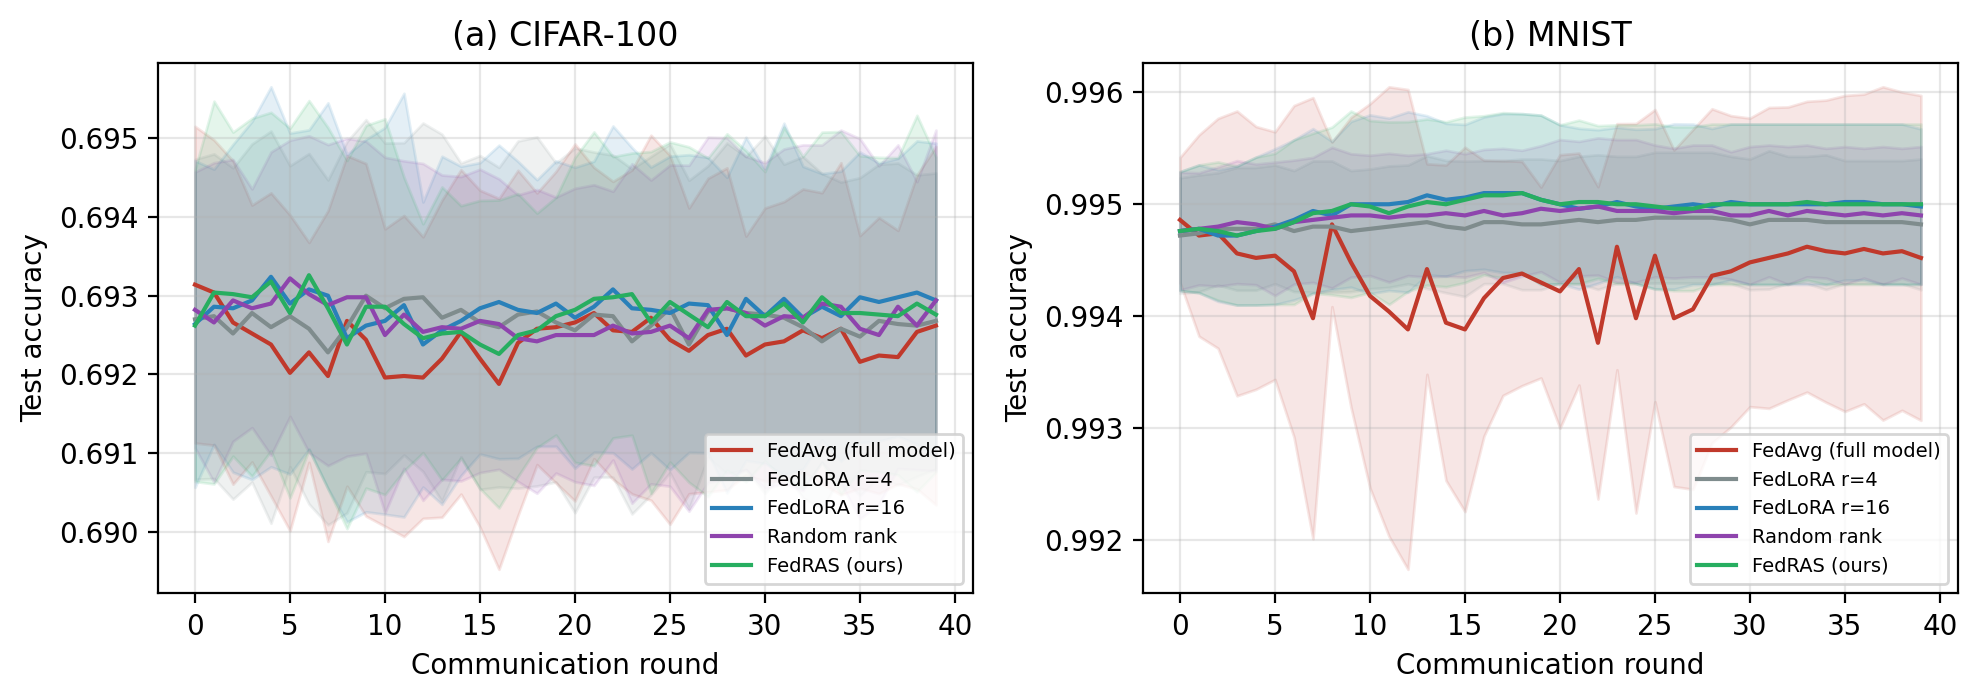
\includegraphics[width=0.8\columnwidth]{cross_dataset.png}
\caption{Cross-dataset test accuracy on CIFAR-100 and MNIST (mean$\pm$std, five seeds). The parity and stability findings of Table~\ref{tab:trainer} are not CIFAR-10-specific.}
\label{fig:crossds}
\end{figure}

\begin{table}[H]
\centering
\caption{Real trainer, non-IID CIFAR-10, nominal deadline (five seeds). Accuracy at round 40; timely ratio and bytes averaged over rounds 30--39 (bytes are the normalized per-round payload summed over the 10 participants); the mean rank is taken over delivered updates; Acc/MB is final accuracy per normalized MB.}
\label{tab:trainer}
\resizebox{0.92\columnwidth}{!}{%
\begin{tabular}{lccccc}
\toprule
Method & Accuracy & Timely ratio & Bytes/round & Mean rank & Acc/MB ($\times10^{-2}$)\\
\midrule
FedAvg (full model) & $0.9138\pm0.0019$ & 0.28 & 17.80 & 64 & 5.1\\
FedLoRA $r{=}4$ & $0.9145\pm0.0012$ & 0.50 & 5.80 & 4 & 15.8\\
FedLoRA $r{=}16$ & $0.9142\pm0.0016$ & 0.44 & 8.20 & 16 & 11.1\\
Random rank & $0.9144\pm0.0016$ & 0.49 & 6.51 & 7.4 & 14.1\\
FedRAS (ours) & $0.9143\pm0.0015$ & 0.44 & 8.14 & 16.0 & 11.2\\
\bottomrule
\end{tabular}%
}
\end{table}

\subsection{Accuracy parity and rank invariance in the trainer}
Table~\ref{tab:trainer} reports five-seed means and standard deviations after 40 federated rounds on CIFAR-10. All LoRA methods hold the backbone accuracy within one standard deviation of 0.914, whether the rank is fixed at 4, fixed at 16, drawn at random, or chosen adaptively. Full-parameter updates also match this accuracy, but they spend 17.8 normalized MB per round against 5.8 to 8.2 for the LoRA ranks, a factor of 2.2 to 3.1. They also lose roughly half of the timely deliveries, 0.28 against 0.44 to 0.50, because their large payloads are dropped more often. The trainer therefore supports a clean parity claim. With a frozen pretrained backbone, the rank costs no measurable accuracy, and what differs across methods is the network bill. The cross-dataset results agree at 0.693 on CIFAR-100 and 0.995 on MNIST. Figs.~\ref{fig:crossds} and \ref{fig:trainer_acc} show the corresponding trajectories, all stable over the 40 rounds for every rank policy.

\begin{figure}[H]
\centering
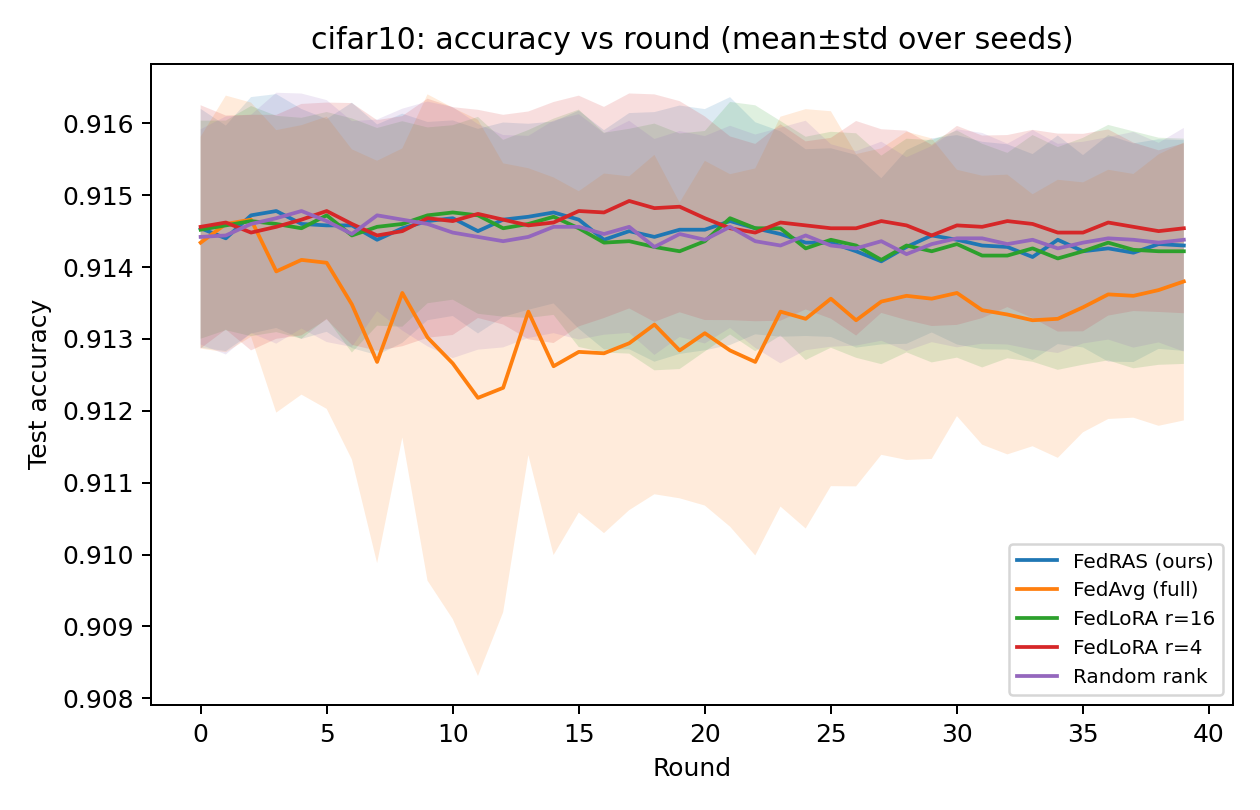
\includegraphics[width=0.8\columnwidth]{trainer_accuracy.png}
\caption{Real-trainer CIFAR-10 test accuracy over 40 federated rounds (mean$\pm$std over five seeds). All rank policies hold the pretrained-backbone accuracy; differences appear in bytes and timeliness, not accuracy.}
\label{fig:trainer_acc}
\end{figure}

\subsection{Deadline stress in the trainer}
Table~\ref{tab:stress} tightens the deadline to 0.5\,s and 0.25\,s with five seeds. It reports accuracy at round 40 and network metrics averaged over rounds 30 to 39. Three effects emerge. First, FedRAS downshifts under pressure. Its delivered mean rank falls from 16.0 at the nominal deadline to 15.5 at 0.5\,s and 13.5 at 0.25\,s, where the delivery hazard \eqref{eq:hazard} makes rank-16 payloads marginal. The loose-deadline control at 2\,s in Table~\ref{tab:extended} restores rank 16.0, so FedRAS upshifts again when pressure is absent. Second, downshifting pays. FedRAS matches the accuracy of fixed $r{=}16$, 0.9145 versus 0.9142, while transmitting 14\% fewer bytes, 7.07 against 8.20\,MB, and delivering the same number of updates per round. Third, full-parameter updates collapse. Their timely ratio falls from 0.28 at the nominal deadline in Table~\ref{tab:trainer} to 0.13 at 0.5\,s and 0.04 at 0.25\,s, so only 0.4 of the 10 updates arrive per round at an unchanged $2.2\times$ byte cost.

\begin{table}[H]
\centering
\caption{Extended stress matrix (five seeds, round-40 accuracy, mean$\pm$std). The loose-deadline and mobility-only scenarios confirm that FedRAS upshifts when pressure is absent; $\alpha{=}0.1$ probes extreme non-IID heterogeneity; the last two columns repeat the 0.25\,s deadline on CIFAR-100 and MNIST. Bold marks the best value at displayed precision, ties included.}
\label{tab:extended}
\resizebox{0.92\columnwidth}{!}{%
\begin{tabular}{l ccccc}
\toprule
Method & dl 2\,s & Mob.\ 0.7 & $\alpha{=}0.1$ & CIFAR-100 dl 0.25\,s & MNIST dl 0.25\,s\\
\midrule
FedAvg (full model) & $0.9128\pm.0026$ & $0.9125\pm.0016$ & $0.9059\pm.0047$ & $0.6924\pm.0021$ & $0.9946\pm.0009$\\
FedLoRA $r{=}4$ & $\mathbf{0.9144\pm.0013}$ & $0.9143\pm.0015$ & $\mathbf{0.9138\pm.0014}$ & $\mathbf{0.6928\pm.0022}$ & $0.9948\pm.0006$\\
FedLoRA $r{=}16$ & $\mathbf{0.9144\pm.0015}$ & $0.9142\pm.0014$ & $0.9109\pm.0026$ & $0.6927\pm.0017$ & $\mathbf{0.9949\pm.0006}$\\
Random rank & $\mathbf{0.9144\pm.0016}$ & $0.9142\pm.0019$ & $\mathbf{0.9140\pm.0018}$ & $\mathbf{0.6928\pm.0020}$ & $\mathbf{0.9949\pm.0007}$\\
FedRAS (ours) & $0.9142\pm.0014$ & $\mathbf{0.9143\pm.0015}$ & $0.9111\pm.0028$ & $0.6925\pm.0020$ & $\mathbf{0.9949\pm.0006}$\\
\bottomrule
\end{tabular}%
}
\end{table}

\begin{table}[H]
\centering
\caption{Real trainer under deadline stress (non-IID CIFAR-10, five seeds). Accuracy at round 40 (mean$\pm$std); timely ratio, bytes, and rank averaged over rounds 30--39; rank is the mean rank of delivered updates.}
\label{tab:stress}
\resizebox{0.92\columnwidth}{!}{%
\begin{tabular}{l cccc cccc}
\toprule
& \multicolumn{4}{c}{deadline 0.5\,s} & \multicolumn{4}{c}{deadline 0.25\,s}\\
\cmidrule(lr){2-5}\cmidrule(lr){6-9}
Method & Acc. & Timely & Bytes & Rank & Acc. & Timely & Bytes & Rank\\
\midrule
FedAvg (full model) & $0.9132\pm.0021$ & 0.13 & 17.80 & 64 & $0.9137\pm.0026$ & 0.04 & 17.80 & 64\\
FedLoRA $r{=}4$ & $0.9142\pm.0013$ & 0.37 & 5.80 & 4 & $0.9147\pm.0019$ & 0.21 & 5.80 & 4\\
FedLoRA $r{=}16$ & $0.9141\pm.0015$ & 0.30 & 8.20 & 16 & $0.9142\pm.0019$ & 0.15 & 8.20 & 16\\
Random rank & $0.9143\pm.0014$ & 0.32 & 6.51 & 6.5 & $0.9148\pm.0017$ & 0.17 & 6.51 & 6.5\\
FedRAS (ours) & $0.9141\pm.0018$ & 0.31 & 7.80 & 15.5 & $0.9145\pm.0020$ & 0.16 & 7.07 & 13.5\\
\bottomrule
\end{tabular}%
}
\end{table}

Accuracy spreads remain within about two standard deviations, which is consistent with the parity claim. The scheduling metrics are where the methods separate. Fig.~\ref{fig:trainer_dl} shows the five-seed stress trajectories. Fig.~\ref{fig:rankdyn} visualizes the mechanism directly. The delivered rank of FedRAS sits at 16 under the nominal deadline, dips under the 0.5\,s deadline, and tracks 10 to 14 under the 0.25\,s deadline, whereas the annealed baseline follows its fixed heat--cool path regardless of link state. A ten-seed replication confirms these differences at conventional significance levels, with full statistics in Section~\ref{sec:summary}. Under the 0.25\,s deadline, FedRAS transmits 14.5\% fewer bytes than fixed $r{=}16$, with a seed-mean bootstrap 95\% confidence interval from 12.4\% to 18.6\% and a two-sided Wilcoxon $p$ of 0.002. It delivers a higher timely ratio in ten of ten seed pairs at $p=0.016$, and it remains statistically indistinguishable in accuracy at $p=0.40$.

\begin{figure}[H]
\centering
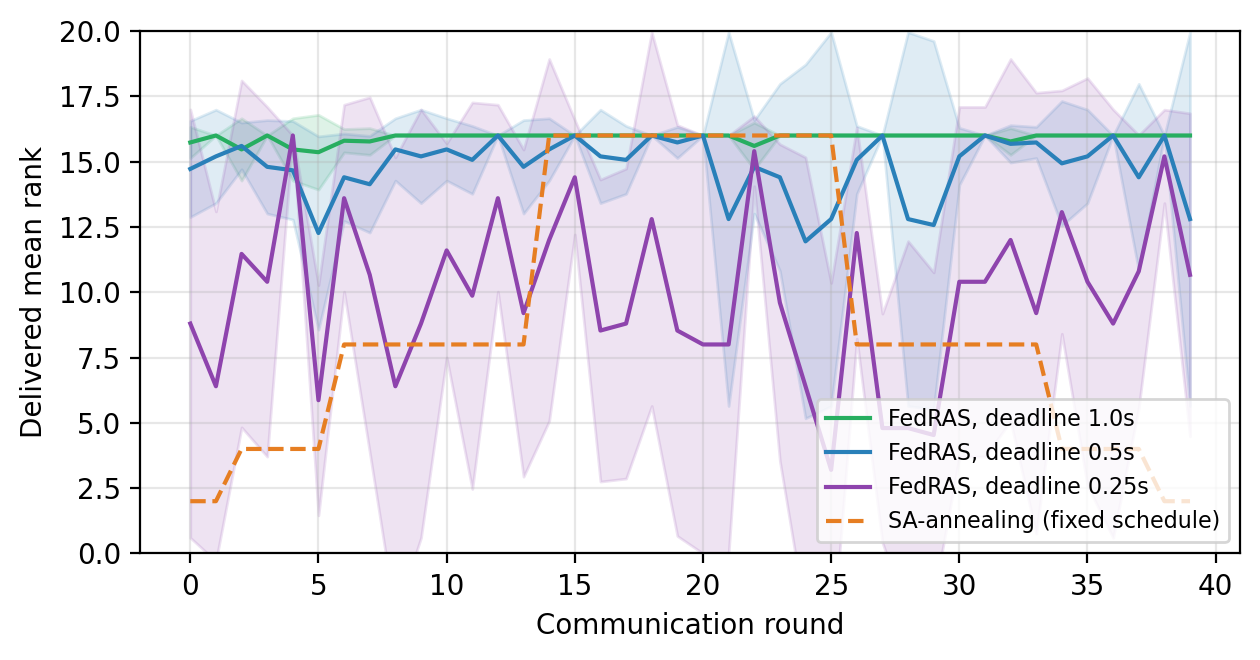
\includegraphics[width=0.8\columnwidth]{rank_dynamics.png}
\caption{Delivered mean rank per round for FedRAS under three deadlines (mean$\pm$std, five seeds), against the fixed annealing schedule of the SA-FedLoRA-style baseline. FedRAS is link-aware, holding high rank when possible and downshifting under pressure.}
\label{fig:rankdyn}
\end{figure}

\begin{figure}[H]
\centering
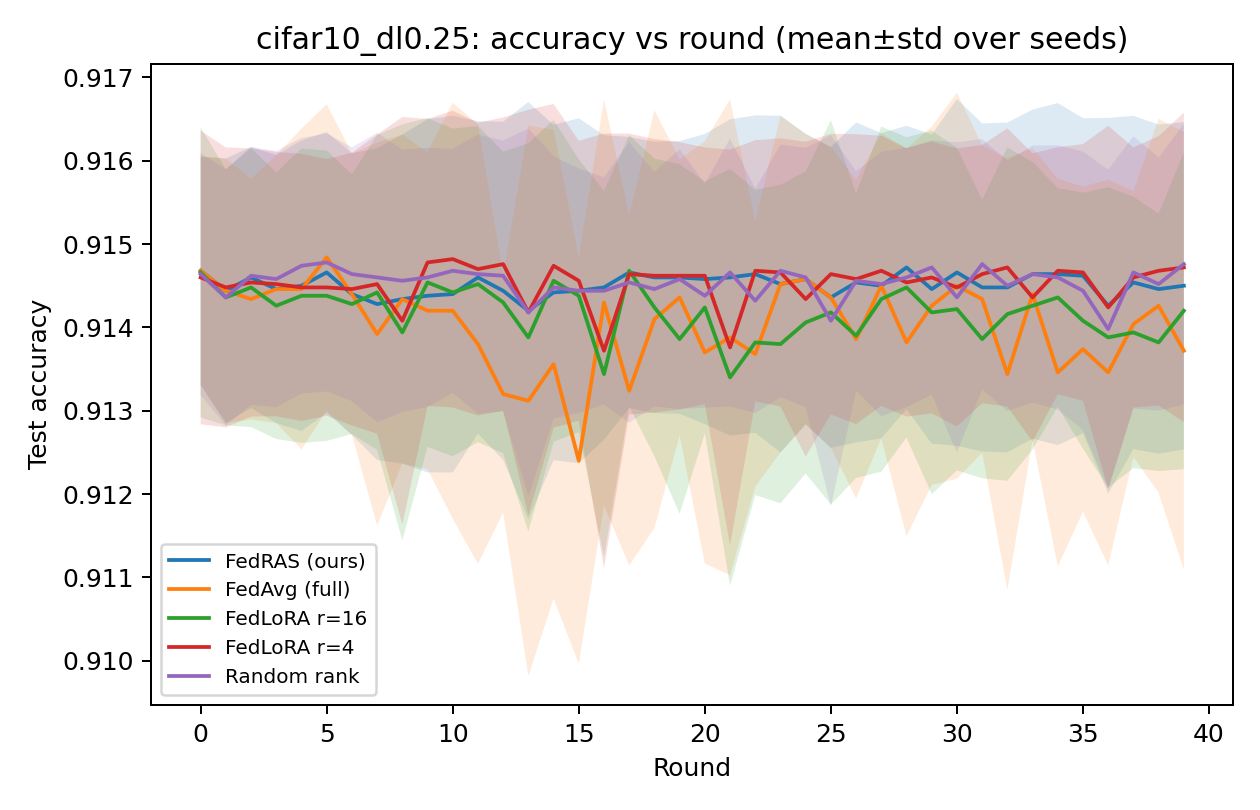
\includegraphics[width=0.8\columnwidth]{trainer_dl025.png}
\caption{Real-trainer accuracy trajectories under the 0.25\,s deadline (mean$\pm$std, five seeds). All methods remain stable. FedRAS selects lower ranks on slow links and matches rank-16 delivery at 14\% fewer bytes.}
\label{fig:trainer_dl}
\end{figure}

\subsection{Broader stress matrix with mobility, heterogeneity, and cross-dataset checks}
Table~\ref{tab:extended} extends the stress study along three further axes. A mobility-only scenario with Beta$(0.7,\,5)$ mobility and the nominal deadline leaves FedRAS at the top rank and at parity, so mobility alone does not force downshifting at this deadline, consistent with the mobility-stress regime of the simulator. Extreme label heterogeneity with $\alpha{=}0.1$ reveals a second-order effect. Rank-16 updates lose about 0.3 points relative to rank 4, 0.9109 versus 0.9138, which is consistent with capacity-amplified client drift, and full-parameter updates lose the most at 0.9059. FedRAS follows the rank-16 trajectory here, so a heterogeneity-aware downshift is a natural extension. Repeating the 0.25\,s deadline on CIFAR-100 and MNIST reproduces the CIFAR-10 stress picture, with parity across LoRA ranks and a timely ratio of 0.04 for full-parameter updates, meaning 0.4 of 10 updates per round. The scheduling conclusions are therefore not dataset-specific.

\subsection{External baselines and component ablations}
Table~\ref{tab:ext} adds three external baselines to the trainer. The first is an SA-FedLoRA-style schedule that heats the rank from 2 to 16 and cools it down over the 40 rounds, oblivious to link state \cite{yang2024safedlora}. The second is an Oort-style selector that samples $2K$ candidates and admits the top-$K$ by a data-size-and-recency utility at fixed rank \cite{oort2021oort}. The third is joint A/B training with plain averaging, the aggregation-level competitor of Section~\ref{sec:aggregation} \cite{guo2025fedsalora}.

\begin{table}[H]
\centering
\caption{External baselines, real trainer (non-IID CIFAR-10, five seeds). Accuracy at round 40; timely ratio, bytes, and delivered mean rank averaged over rounds 30--39.}
\label{tab:ext}
\resizebox{\columnwidth}{!}{%
\begin{tabular}{l cccc cccc}
\toprule
& \multicolumn{4}{c}{nominal deadline} & \multicolumn{4}{c}{deadline 0.25\,s}\\
\cmidrule(lr){2-5}\cmidrule(lr){6-9}
Method & Acc. & Timely & Bytes & Rank & Acc. & Timely & Bytes & Rank\\
\midrule
SA-FedLoRA-style annealing & $0.9145\pm.0016$ & 0.49 & 6.04 & 5.2 & $0.9146\pm.0016$ & \textbf{0.20} & \textbf{6.04} & 4.8\\
Oort-style utility, fixed rank & $0.9141\pm.0017$ & 0.49 & 6.60 & 8.0 & $0.9142\pm.0013$ & 0.18 & 6.60 & 6.4\\
Joint A/B, plain averaging & $0.9143\pm.0015$ & 0.44 & 8.20 & 16 & $0.9140\pm.0017$ & 0.15 & 8.20 & 12.5\\
\midrule
FedLoRA $r{=}16$ & $0.9142\pm.0016$ & 0.44 & 8.20 & 16 & $0.9142\pm.0019$ & 0.15 & 8.20 & 12.5\\
FedRAS (ours) & $0.9143\pm.0015$ & 0.44 & 8.14 & 16.0 & $0.9145\pm.0020$ & 0.16 & 7.07 & 13.5\\
\bottomrule
\end{tabular}%
}
\end{table}

\begin{table}[H]
\centering
\caption{Scheduler simulation, 500 clients, 150 rounds, five seeds, final round. Accuracy is the bounded scheduling proxy (not dataset accuracy); bytes are per-round totals over admitted clients.}
\label{tab:sim}
\resizebox{0.92\columnwidth}{!}{%
\begin{tabular}{lccc ccc ccc ccc}
\toprule
& \multicolumn{3}{c}{Nominal} & \multicolumn{3}{c}{Deadline 0.25\,s} & \multicolumn{3}{c}{Budget 12 MB} & \multicolumn{3}{c}{1000 clients}\\
\cmidrule(lr){2-4}\cmidrule(lr){5-7}\cmidrule(lr){8-10}\cmidrule(lr){11-13}
Method & Acc. & Timely & Bytes & Acc. & Timely & Bytes & Acc. & Timely & Bytes & Acc. & Timely & Bytes\\
\midrule
FedAvg & .607 & .26 & 44.5 & .187 & .04 & 44.5 & .397 & .43 & 10.7 & .577 & .35 & 58.7\\
$r{=}4$ & .606 & .51 & 14.5 & .343 & .20 & 14.5 & .576 & .54 & 11.6 & .610 & .51 & 29.0\\
$r{=}16$ & \textbf{.778} & .44 & 20.5 & .404 & .14 & 20.5 & \textbf{.687} & .52 & 11.5 & \textbf{.781} & .44 & 41.0\\
Random & .666 & .48 & 16.5 & .359 & .18 & 16.5 & .620 & .52 & 11.9 & .668 & .48 & 32.9\\
Reliability-only & .508 & .52 & 13.5 & .292 & .22 & 13.5 & .493 & .55 & 11.9 & .511 & .52 & 27.0\\
FedRAS (ours) & \textbf{.778} & .44 & 20.3 & \textbf{.413} & .15 & 17.8 & \textbf{.687} & .52 & 11.5 & \textbf{.781} & .44 & 40.7\\
\bottomrule
\end{tabular}%
}
\end{table}

On accuracy, every method remains within noise of the backbone, as the parity claim predicts. The informative differences are structural, and they differ by regime. Under the 0.25\,s deadline the annealed schedule happens to sit at low rank, so it delivers the most updates per round, 2.0 against 1.6 for FedRAS, at the fewest bytes. The schedule is fixed a priori, however, and cannot upshift when links allow. The capacity-aware simulator makes this cost visible. The same schedule settles at rank 2 and loses 8.2 points of scheduling accuracy to FedRAS in the nominal regime, 0.696 against 0.778, and 3.9 points under stress, 0.374 against 0.413, as Table~\ref{tab:sim} shows.

The other two baselines show the same pattern. The Oort-style selector concentrates participation on high-utility clients but cannot trade capacity against delivery at fixed rank. Joint A/B training matches frozen-factor training at the adopted learning rate, and its cost appears under drift pressure in the ablation below.

A ten-seed replication of the three baselines under both deadlines confirms this picture at conventional significance levels. Accuracy parity holds throughout, with a largest mean difference of 0.03 percentage points and all $p\ge0.09$. The annealed schedule reaches higher timely ratios at fewer bytes, exactly as its fixed low-rank path predicts, with $p\le0.004$. Oort-style selection saves bytes at parity with $p=0.002$. Joint A/B matches frozen-factor training in accuracy while losing timely deliveries to FedRAS under stress, by 0.019 at $p=0.016$.

\begin{table}[H]
\centering
\caption{Component ablations, real trainer (non-IID CIFAR-10, five seeds, nominal deadline). The Min. column is the minimum per-seed-mean accuracy over rounds, reported for the elevated-learning-rate stability check at lr $0.02$.}
\label{tab:ablation}
\resizebox{\columnwidth}{!}{%
\begin{tabular}{l cccc c}
\toprule
Configuration & Acc. & Timely & Bytes & Rank & Min.\\
\midrule
Full system (ours) & $0.9143\pm.0015$ & 0.44 & 8.14 & 16.0 & ---\\
\midrule
w/o capacity term & $0.9145\pm.0015$ & \textbf{0.52} & \textbf{5.40} & 2.0 & ---\\
w/o frozen A (joint A/B) & $0.9143\pm.0015$ & 0.44 & 8.20 & 16.0 & ---\\
w/o rank mask (mixed-rank rounds) & $0.9145\pm.0016$ & 0.49 & 6.51 & 7.4 & ---\\
w/o server momentum & $0.9144\pm.0016$ & 0.44 & 8.14 & 16.0 & ---\\
\midrule
frozen A, lr $0.02$ & $0.9128\pm.0017$ & --- & --- & --- & \textbf{0.909}\\
joint A/B, lr $0.02$ & $0.9127\pm.0017$ & --- & --- & --- & 0.901\\
\bottomrule
\end{tabular}%
}
\end{table}

Table~\ref{tab:ablation} reports component ablations. In the parity regime, no removal measurably changes final accuracy, which is consistent with the claim that accuracy is carried by the backbone and not by the scheduler. The components instead shape network behavior and stability margins. Removing the capacity term collapses FedRAS to rank 2, with 5.40 bytes and delivered rank 2.0. Delivery-only optimization is the degenerate policy that the capacity term exists to prevent. Its capacity cost is invisible at nominal deadlines but material in the simulator, where rank 2 loses 27 points of scheduling accuracy to rank 16, as Table~\ref{tab:sim} shows.

Removing the frozen-factor property does not hurt at the adopted learning rate. At an elevated rate of 0.02, joint A/B training shows a markedly deeper transient accuracy dip before recovering, with a minimum of 0.901 against 0.909 across rounds and seeds, which matches the factor-rotation analysis of Section~\ref{sec:aggregation}. The rank mask and server momentum are accuracy-neutral here, because at the adopted operating point all clients often share one rank and the momentum is small. The mask is nonetheless what keeps heterogeneous-rank aggregation per-slice exact whenever ranks mix, as Proposition~\ref{prop:agg} states.

\subsection{Full scheduling versus fair-cohort in the trainer}
\label{sec:dpvfair}
The trainer results so far use fair-cohort scheduling, that is, uniform sampling plus a per-client rank argmax. The exact client--rank DP, by contrast, has so far been exercised only in the simulator. We therefore add a full-scheduling arm to the trainer. Each round, this arm solves the exact DP of Section~\ref{sec:solver} over the entire 20-client population, so both arms see the same candidate set. Both arms share the participation cap $K{=}10$, and the DP arm additionally enforces a byte budget of 8.2\,MB, which is $10\times$ the rank-16 payload, so the budget binds only through downshifting or skipping. The budget grid is the 0.05\,MB grid of the solver study.

\begin{table}[H]
\centering
\caption{Full scheduling versus fair-cohort in the real trainer (non-IID CIFAR-10, nominal deadline, ten seeds): accuracy at round 40; network metrics averaged over rounds 30--39. Both arms share the candidate set (all 20 clients) and the participation cap $K{=}10$; the DP arm additionally enforces an 8.2\,MB byte budget.}
\label{tab:dpvfair}
\resizebox{\columnwidth}{!}{%
\begin{tabular}{lcccc}
\toprule
Method & Accuracy & Timely ratio & Bytes/round & Mean rank\\
\midrule
Full DP (exact assignment, 8.2\,MB) & $\mathbf{0.9152\pm.0016}$ & $\mathbf{0.56}$ & $\mathbf{7.88}$ & 14.7\\
Fair cohort (FedRAS rule) & $0.9151\pm.0016$ & 0.42 & 8.13 & 15.9\\
FedLoRA $r{=}16$ & $0.9150\pm.0017$ & 0.42 & 8.20 & 16\\
\bottomrule
\end{tabular}%
}
\end{table}

Table~\ref{tab:dpvfair} reports ten seeds. The DP arm matches accuracy exactly, 0.9152 versus 0.9151 at $p=0.75$, while delivering strictly better network behavior than fair-cohort. Its timely ratio is 0.56 against 0.42 at $p=0.002$, at 3\% fewer bytes, also at $p=0.002$. It achieves this by admitting link-favoured clients and downshifting where the budget binds, with a delivered mean rank of 14.7 versus 15.9. This is the objective gap made physical. Fair-cohort buys population-fair participation at a measurable timeliness cost, and the exact assignment transfers from the simulator to real training without modification.

\subsection{Scheduler behavior at 500-client scale}
Table~\ref{tab:sim} summarizes the simulator across regimes, with five seeds at the final round, and the full nine-regime matrix is provided in the reproducibility package. In the nominal regime, FedRAS matches the best fixed rank at 0.778 at slightly fewer bytes. Both outperform random rank at 0.666, rank 4 at 0.606, and FedAvg-style rank-64 updates at 0.607 and $2.2\times$ the bytes. Under deadline stress the separation grows. At 0.25\,s, FedRAS reaches 0.413 versus 0.404 for fixed $r{=}16$, 0.359 for random, and 0.374 for the link-oblivious annealed schedule, while full-parameter updates fall to 0.187 and their timely ratio collapses to 0.037. Under the binding 12\,MB budget, FedRAS and fixed $r{=}16$ tie at 0.687 because the cap rather than the rank binds, while full-parameter updates fall to 0.397. The mobility-stress and 1000-client regimes show the same pattern at fewer bytes. Across all nine regimes, FedRAS is best or statistically tied for best.

\begin{figure}[H]
\centering
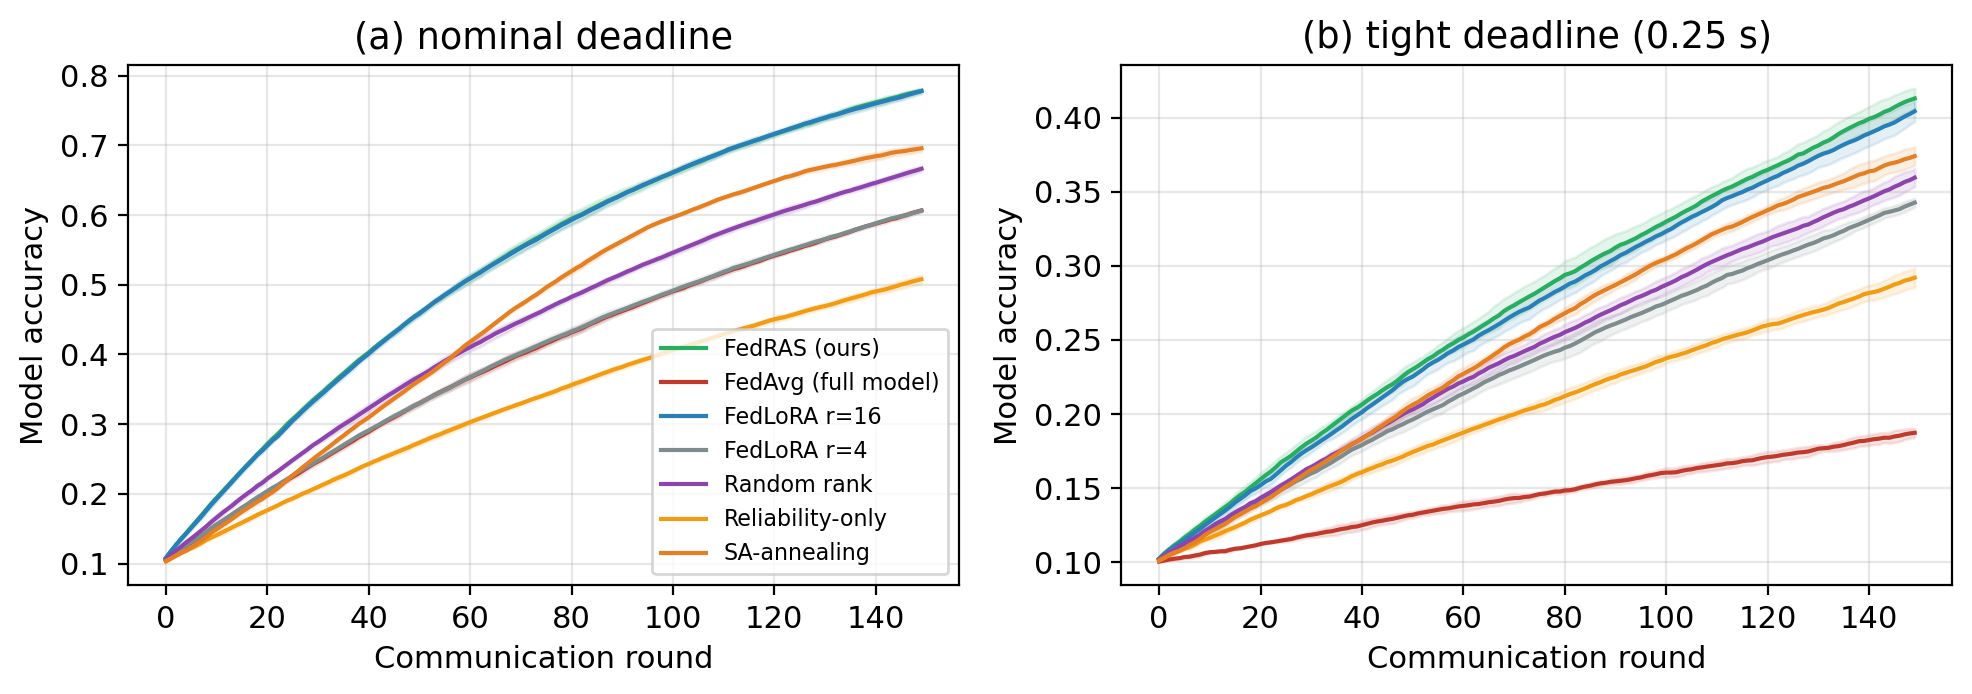
\includegraphics[width=0.8\columnwidth]{sim_accuracy.png}
\caption{Scheduler simulation accuracy trajectories (mean$\pm$std, five seeds). Under the nominal deadline (left) FedRAS matches fixed rank 16. Under the 0.25\,s deadline (right) FedRAS downshifting separates from fixed rank 16 and outperforms random and full updates.}
\label{fig:sim}
\end{figure}

\begin{figure}[H]
\centering
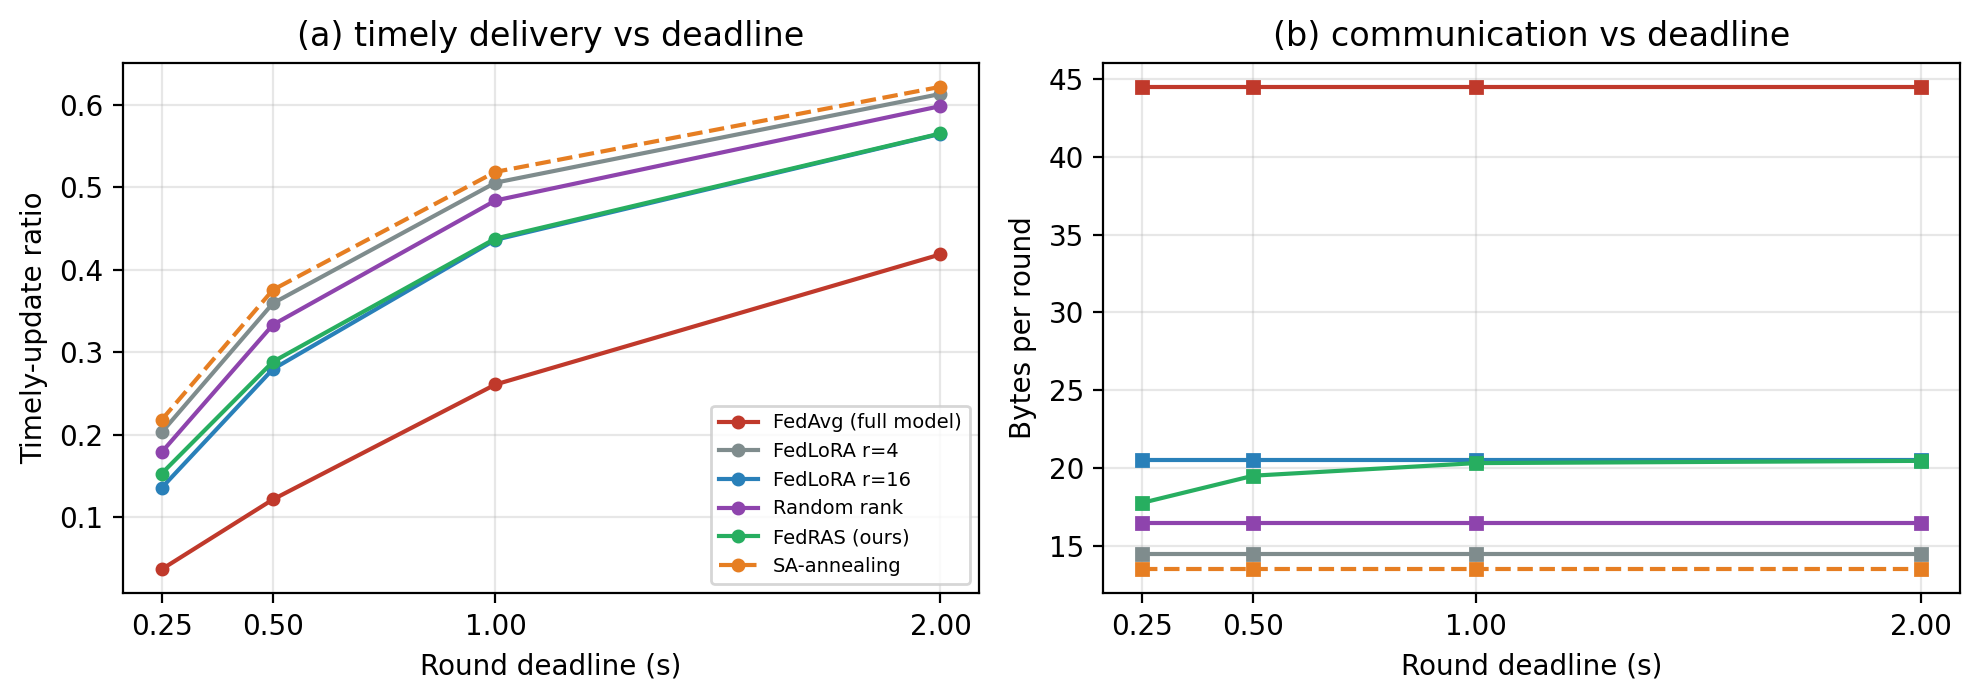
\includegraphics[width=0.8\columnwidth]{sim_deadline.png}
\caption{Simulator network view with timely delivery and per-round bytes versus the round deadline (500 clients, five seeds). Full updates collapse on the delivery axis. The annealed schedule and reliability-only policies save bytes only by giving up rank everywhere, regardless of link state.}
\label{fig:simdl}
\end{figure}

Fig.~\ref{fig:sim} shows the nominal and 0.25\,s trajectories, and Fig.~\ref{fig:simdl} shows the network-side view. Full-parameter updates lose 86\% of their timely deliveries as the deadline tightens from the nominal deadline to 0.25\,s at a constant $2.2\times$ byte cost. The annealed schedule buys timely delivery by settling at rank 2, and FedRAS tracks fixed rank 16 on both accuracy and timely delivery at 14\% fewer bytes.

\begin{table}[H]
\centering
\caption{Solver study (500 clients, $K{=}25$, 30 instances per cell): optimality gap of heuristics relative to the exact DP, and DP runtime.}
\label{tab:dp}
\resizebox{\columnwidth}{!}{%
\begin{tabular}{cc ccc c}
\toprule
Deadline (s) & Budget (MB) & Greedy val/byte & Greedy value & Fixed $r{=}16$ & DP time (ms)\\
\midrule
1.0  & 300 & 0.0\% & 0.0\% & 0.0\% & 836\\
1.0  & 40  & 0.0\% & 0.0\% & 0.0\% & 92\\
1.0  & 12  & 6.1\% & 6.1\% & 6.1\% & 33\\
0.5  & 300 & 0.7\% & 0.0\% & 0.0\% & 833\\
0.5  & 40  & 0.8\% & 0.0\% & 0.0\% & 92\\
0.5  & 12  & 5.6\% & 6.0\% & 6.0\% & 33\\
0.25 & 300 & \textbf{9.7\%} & 0.0\% & 0.0\% & 830\\
0.25 & 40  & \textbf{10.0\%} & 0.0\% & 0.0\% & 92\\
0.25 & 12  & 4.5\% & 5.8\% & 5.8\% & 33\\
\bottomrule
\end{tabular}%
}
\end{table}

\subsection{Solver optimality and runtime}
\label{sec:dp_study}
Table~\ref{tab:dp} reports the scheduling study. When the byte budget is slack, greedy heuristics are near-optimal and the choice of scheduler matters little. The interesting regimes are the binding ones. When the budget binds at 12\,MB, value-per-byte greedy loses 4.5 to 6.1\% of the expected useful updates, and under a tight deadline it loses up to 10\% even when the budget is slack, with 9.7\% at 300\,MB and 10.0\% at 40\,MB, because per-byte ordering misprices delivery risk. The exact DP attains the optimum in every cell. Its runtime is 33 to 836\,ms for 500 clients depending on the budget-grid size, which the 0.05\,MB grid dominates, and it scales linearly to 1000 clients, as Fig.~\ref{fig:dp} shows. This is compatible with per-round scheduling at minute-scale FL rounds, and the grid step offers a tuning knob.

\begin{figure}[H]
\centering
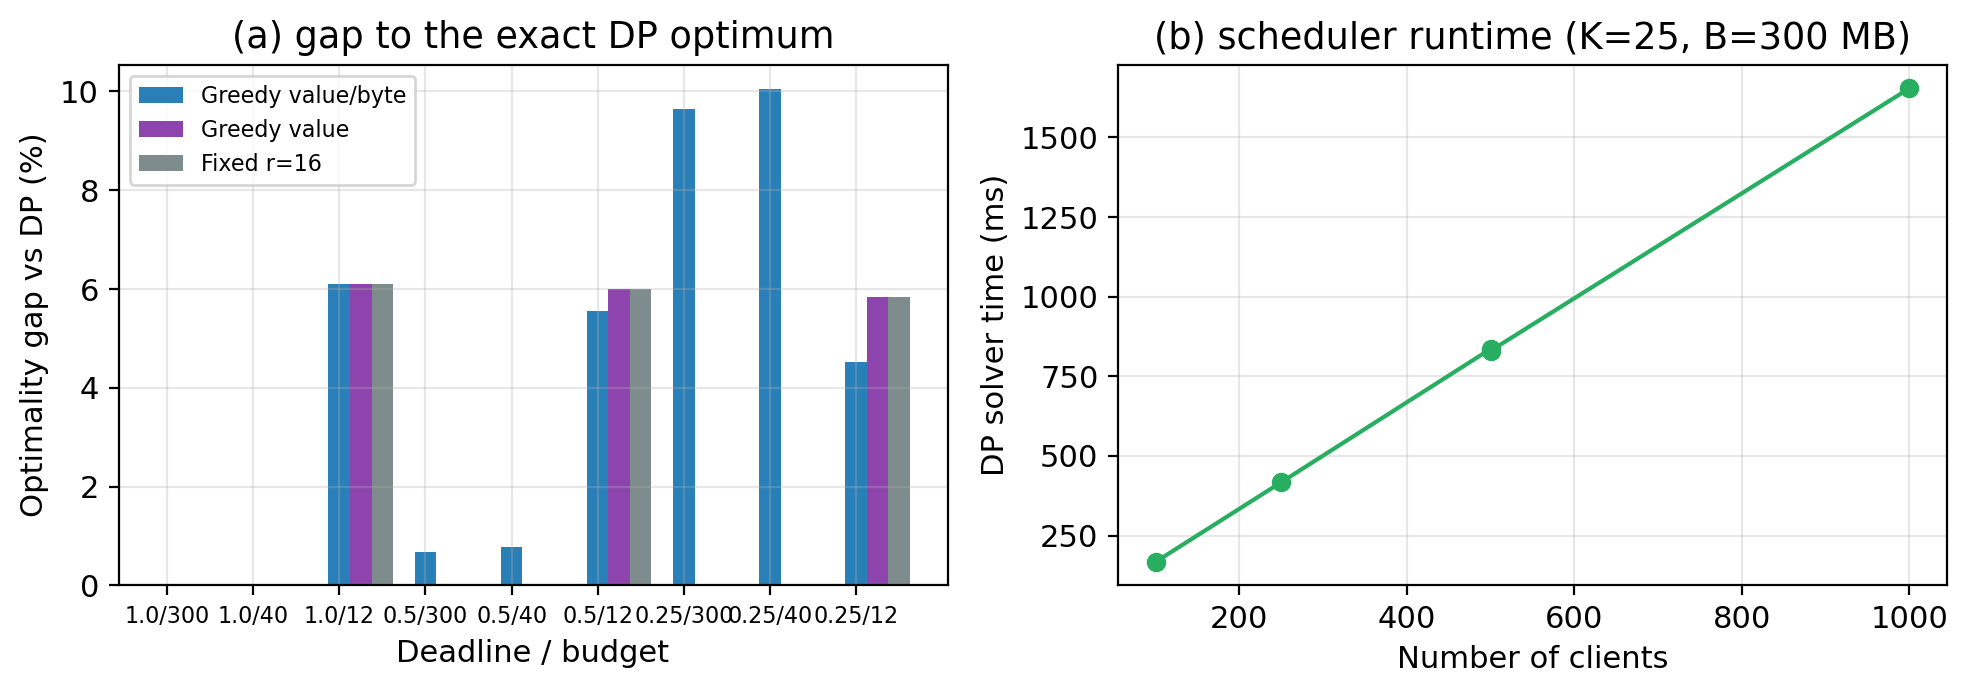
\includegraphics[width=0.8\columnwidth]{dp_study.png}
\caption{Solver study. The left panel shows the optimality gap of greedy heuristics versus the exact DP across deadline and budget cells, where per-byte greedy degrades up to 10\% when the budget binds or the deadline is tight. The right panel shows the DP runtime, which grows linearly with the client population from 167\,ms at 100 clients to 1654\,ms at 1000.}
\label{fig:dp}
\end{figure}

A dedicated grid sweep with steps from 0.2 to 0.01\,MB and 30 instances per cell compares each step against a 0.01\,MB reference. When the budget is slack, the objective is step-insensitive, with 0\% deviation at every step. In the binding 12\,MB regime, the default 0.05\,MB step shifts the objective by at most 3.3\% across instances and deadlines, and a 0.025\,MB step bounds the deviation to 1.3\% at $1.7\times$ the runtime, that is, 27 to 45\,ms per round at 500 clients. The optimality claim of Section~\ref{sec:solver} therefore holds on a grid whose quantization error is bounded, measured, and adjustable at a known runtime cost. The fair-cohort variant used by the trainer, uniform sampling plus per-client argmax, reaches 27 to 55\% of the unconstrained DP objective. This is the price of population-fair participation rather than a defect of the FedRAS rank rule, and it delimits when full scheduling is worth its coordination cost.

\begin{figure}[H]
\centering
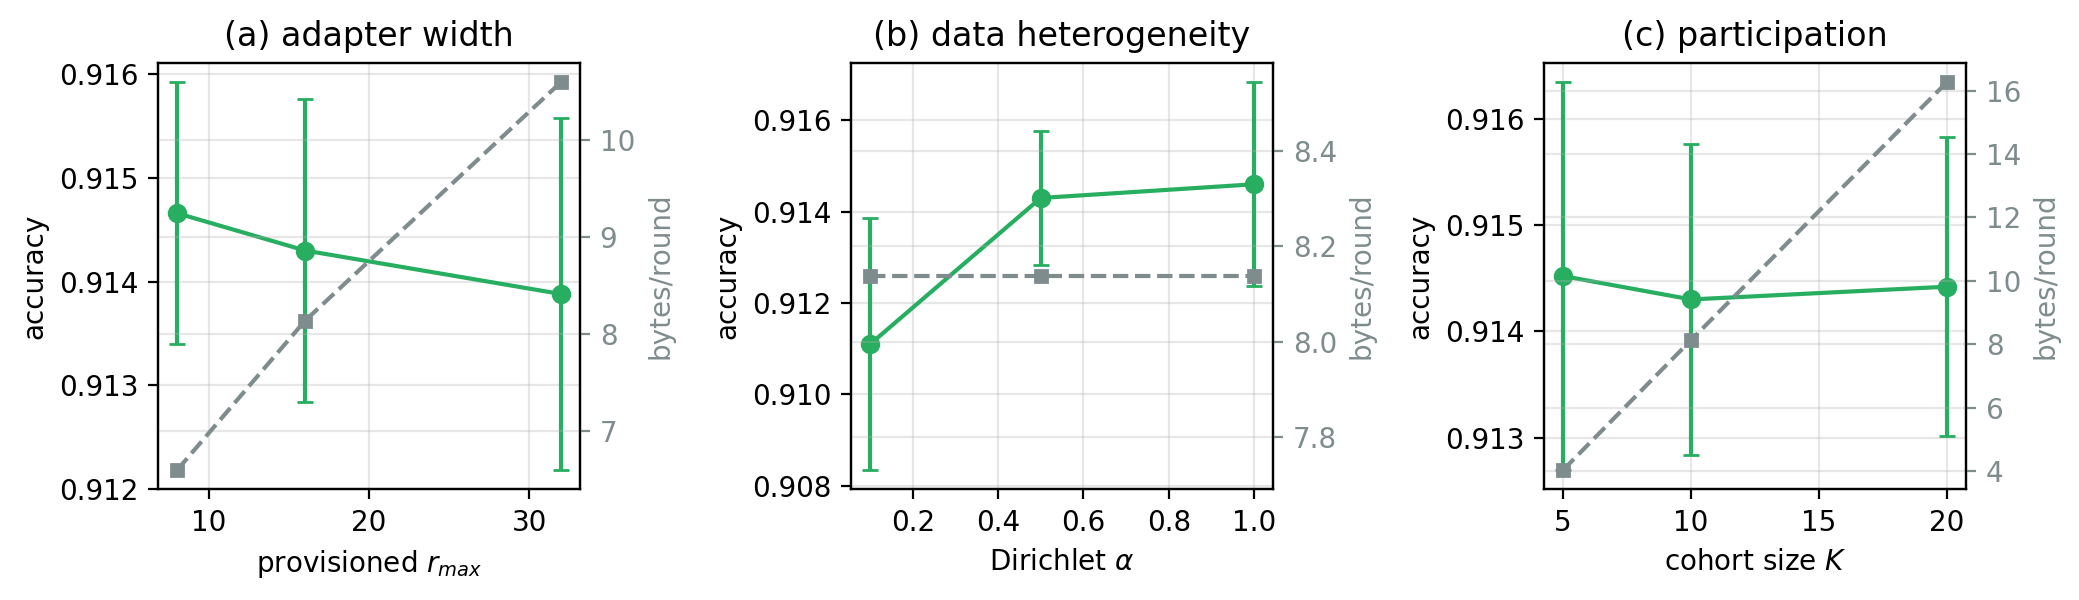
\includegraphics[width=0.98\columnwidth]{sensitivity.png}
\caption{Sensitivity of the trainer to the provisioned adapter width, label heterogeneity, and cohort size (CIFAR-10, FedRAS, five seeds; bars are $\pm$1\,std). Accuracy is flat in $r_{\max}$ and $K$ across the tested ranges; their effect is on bytes and delivered updates.}
\label{fig:sens}
\end{figure}

\subsection{Sensitivity analysis}
Fig.~\ref{fig:sens} varies the provisioned adapter width, the label heterogeneity, and the cohort size of the trainer on CIFAR-10 with five seeds. Widening the adapter from $r_{\max}=8$ to 32 leaves accuracy flat, while bytes rise from 6.6 to 10.6 and delivered updates fall from 4.8 to 3.9 per round. The provisioned width is therefore a network-facing decision rather than an accuracy control. Data heterogeneity from $\alpha=0.1$ to 1.0 moves accuracy from 0.911 to 0.915 at constant network cost, consistent with the parity claim across partitions. Cohort size $K$ from 5 to 20 leaves accuracy flat, while delivered updates grow from 2.3 to 8.6 per round at linearly scaled bytes. At the 0.25\,s deadline, the same growth is throttled by delivery, as the stress results above show. Per-decision scheduling cost is negligible in all settings. The per-client rank rule of the trainer costs 105\,$\mu$s per client--rank decision, about 1\,ms per round, against 33 to 836\,ms for the exact full-scheduling DP of Section~\ref{sec:dp_study}.

\textbf{Robustness to model error.} Two further simulation studies probe how much the scheduler depends on its own estimates. Injecting multiplicative lognormal noise with $\sigma=0.2$ into the predicted $\hat P_{\rm on}$ degrades the achieved objective by at most 5.1\% on average and 9.4\% in the worst instance, and only in the tightest deadline and budget cell. The slack regimes stay below 1\%. Mis-prediction therefore costs optimality smoothly rather than catastrophically, and the observed delivery outcomes of Algorithm~\ref{alg:scheduler} are exactly the signal a calibrated predictor would re-fit.

Replacing the square-root capacity form $G(r)$ with linear or logarithmic alternatives changes admission decisions by at most 0.5\% and the objective by at most 1.4\%. The value of the scheduler thus comes from coupling capacity with delivery risk, not from the specific saturating shape. The sublinear shape itself has an empirical anchor in the trainer, where the mean delivered update norm grows from rank 4 to rank 16 by $1.57\times$, which shows the diminishing returns the square-root model assumes and stays clearly below the $4\times$ linear scaling.

\begin{figure}[H]
\centering
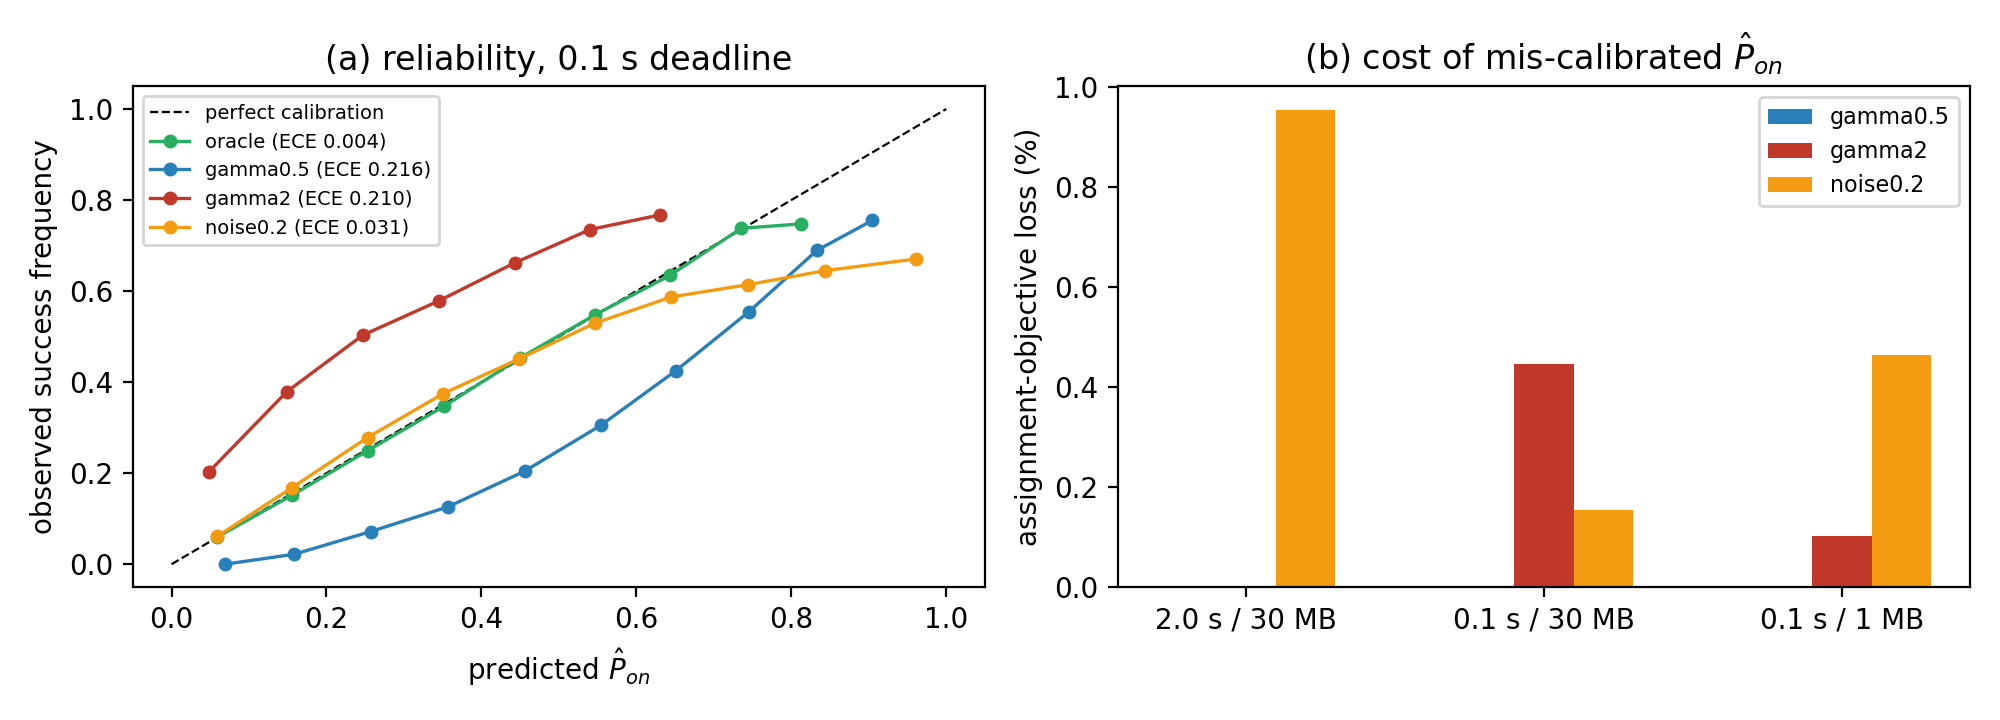
\includegraphics[width=0.8\columnwidth]{fig_calibration.png}
\caption{Delivery-predictor calibration study (500 clients, 150 round-instances per cell). The left panel shows reliability at the 0.25\,s deadline. With oracle link state the hazard-form predictor is calibrated by construction, while the power-distorted ($\gamma$) and noisy variants are measurably miscalibrated. The right panel shows the assignment-objective loss of optimizing against the distorted predictor, evaluated under true probabilities, at most 1.8\% and only in the tightest cell.}
\label{fig:calib}
\end{figure}

\textbf{Calibration of the delivery predictor.} Calibration itself is measurable, and its scheduling cost is bounded, as Fig.~\ref{fig:calib} shows. On the link model of Section~\ref{sec:model}, the deployed predictor with oracle link state is calibrated by construction, with an expected calibration error of 0.002 to 0.004. Deliberately mis-calibrated variants $\hat P^{\gamma}$ with $\gamma$ of 0.5 and 2 reach an error up to 0.21, and multiplicative state noise with $\sigma=0.2$ up to 0.035. The resulting assignment-objective loss, however, stays at most 1.8\% and is confined to the tightest deadline and budget cell, with at most 0.5\% elsewhere. Even sizeable miscalibration therefore leaves the rank ordering largely intact, and the observed outcomes expose it for per-client recalibration. Calibration on measured traces remains open and is taken up in Section~\ref{sec:discussion}.

\subsection{Summary of findings}
\label{sec:summary}
Across the two tiers, a consistent picture emerges. First, rank choice did not measurably change accuracy for this frozen backbone and 40-round horizon, so at this operating point the scheduling freedom is free on the learning side. Second, the network side is where methods differ. Full-parameter updates cost $2.2$ to $3.1\times$ the bytes, and they lose 54\% of their timely deliveries at 0.5\,s, 86\% at 0.25\,s, and 86\% in the simulation as deadlines tighten.

Third, FedRAS behaves as designed, with maximum rank on healthy links, downshifts under pressure, and the top rank again when the deadline is loose. It converts link heterogeneity into a 14\% byte saving while matching fixed rank 16 on accuracy and delivery under stress. Run end to end in the trainer, a full-scheduling DP arm with the same cap and an 8.2\,MB budget lifts the timely ratio from 0.42 to 0.56 at unchanged accuracy over ten seeds at $p=0.002$, so the exact assignment transfers beyond the simulator. Fourth, exactness is affordable, with sub-second per-round solving at 500 clients and material optimality gains precisely in the binding-budget and tight-deadline regimes where greedy scheduling degrades.

The statistical evidence rests on a ten-seed replication of the two headline trainer regimes, over seeds 0 to 9 with common random numbers within each seed. Versus fixed $r{=}16$ under the 0.25\,s deadline, FedRAS saves 14.5\% of bytes at the seed mean, with a bootstrap 95\% confidence interval from 12.4\% to 18.6\%, a two-sided Wilcoxon $p$ of 0.002, and a matched-pairs rank-biserial of magnitude 1.0. It delivers a higher timely ratio in ten of ten seed pairs at $p=0.016$, while the accuracy difference is insignificant at $p=0.40$, and at $p=0.30$ under the nominal deadline.

Versus full-parameter updates the network-side differences are extreme, with 54\% and 61\% fewer bytes at the nominal and stress deadlines at $p=0.002$. The three external baselines replicate at ten seeds with accuracy parity and unchanged network-side structure. With five seeds alone, none of these tests could fall below $p=0.0625$. The statistically supported claims are thus exactly the ones made. They concern network-side savings and accuracy parity, and they do not claim accuracy dominance anywhere.

\section{Discussion and limitations}
\label{sec:discussion}
\textbf{Scope of claims.} The trainer demonstrates parity and not rank-dependent accuracy gains. With a strong frozen backbone and 40 adaptation rounds, transmitted rank does not measurably change test accuracy. Claims that low rank limits adaptation quality would require longer horizons, weaker backbones, or distribution-shifted clients. The simulator capacity model is a scheduling abstraction, and its accuracy is a bounded scheduling proxy rather than a measured dataset accuracy.

\textbf{Backbone pretraining.} The centralized pretraining stage is a documented premise inherited from parameter-efficient FL practice; the federated phase adapts but does not train the backbone. Where no server-side corpus exists, self-supervised or public-data pretraining would be needed, and the parity result should be re-verified.

\textbf{Estimator assumptions.} The hazard-form delivery model \eqref{eq:hazard} assumes the closed-form exponential realization. Production deployments should calibrate $P_{\rm on}$ per client from observed outcomes, for example with isotonic or Platt scaling monitored by a Brier score, and the scheduler treats the predictor as a plug-in.

\textbf{Myopia.} The DP is exact for the estimated per-round problem, not for the multi-round stochastic control problem induced by budget carry-over and mobility correlation; a horizon-aware policy could shift admissions across rounds and is a natural extension.

\textbf{Security.} This work schedules communication and does not propose protection, so we make no privacy claim. Frozen-factor training incidentally reduces the dimensionality of transmitted gradients, which shrinks the gradient-inversion surface. Formal statements require differential-privacy accounting or secure aggregation, which compose orthogonally with rank scheduling \cite{bonawitz2017secureagg,wei2023pfl_dp}.

A further observation from the stress matrix is that under extreme heterogeneity of $\alpha{=}0.1$, higher ranks lose a small amount of accuracy relative to rank 4, consistent with capacity-amplified client drift. The capacity term $G(r)$ could be conditioned on measured heterogeneity to capture this effect, which we leave as future work.

\textbf{Generality.} The trainer validates adapters on convolutional and linear layers of a CNN at $r_{\max}{=}16$ with 20--1000 clients and synthetic link traces. Extension to transformer backbones, measured rather than synthetic links, and larger rank sets changes constants, such as the payload slope and the capacity curve, but not the formulation.

\section{Conclusion}
\label{sec:conclusion}
This paper reframed Federated LoRA over mobile edge networks as a deadline-aware client--rank scheduling problem in which the LoRA rank is a network-visible resource. We derived a rank-dependent delivery model with an explicit MB-to-Mbit hazard, formulated the per-round assignment as a multiple-choice knapsack under budget and participation caps, solved it exactly with a pseudo-polynomial dynamic program, and stabilized heterogeneous-rank aggregation with frozen-factor rank-masked averaging.

Experiments with a real federated LoRA trainer and a 500-client scheduling simulator show that FedRAS preserves backbone accuracy, saves 14\% of update bytes while matching fixed rank 16 on accuracy and delivery under five-seed deadline stress, and exposes the collapse of full-parameter updates, which cost $2.2\times$ the bytes and deliver only 4\% of updates on time at a 0.25\,s deadline. The exact scheduler recovers up to 10\% expected useful updates over greedy heuristics in binding regimes at sub-second cost. Future work includes horizon-aware stochastic scheduling, calibrated per-client delivery predictors, protection mechanisms composed with rank scheduling, and validation on measured mobile traces and transformer backbones.

\section*{Declaration of competing interest}
The authors declare that they have no known competing financial interests or personal relationships that could have appeared to influence the work reported in this paper.

\section*{Acknowledgements}
The authors thank the members of the Information Engineering University research group for many useful discussions and for hands-on assistance with the experimental implementation.

\section*{Funding}
This research did not receive any specific grant from funding agencies in the public, commercial, or not-for-profit sectors.

\section*{CRediT authorship contribution statement}
\textbf{Wenyu Ma:} Methodology, Software, Validation, Investigation, Writing -- original draft.
\textbf{Tao Hu:} Conceptualization, Formal analysis, Supervision, Writing -- review and editing.
\textbf{Xinlei Liu:} Data curation, Investigation, Visualization.
All authors approved the submitted version and accept responsibility for the work.

\section*{Data availability}
The reproducibility package accompanying this submission contains the complete source code (trainer, simulator, solver, and analysis scripts), per-run configuration files, per-seed result tables, and the raw training logs supporting every table and figure in this study; a permanent repository DOI will be supplied at publication.

\section*{Declaration of generative AI and AI-assisted technologies in the manuscript preparation process}
During the preparation of this work the authors used AI-assisted tools for language editing and formatting support. The authors reviewed and edited all generated material and take full responsibility for the content of the published article.

\bibliographystyle{elsarticle-num}
\bibliography{references}
\end{document}
